\chapter{Reliable Data with AI Weather Models}

% **************************** Define Graphics Path **************************
\ifpdf
    \graphicspath{{Chapter3/Figs/}{Chapter3/Figs/PDF/}{Chapter3/Figs/}}
\else
    \graphicspath{{Chapter3/Figs/Vector/}{Chapter3/Figs/}}
\fi

\noindent\textit{The research presented in this chapter was the final component of the dissertation to be undertaken and, unlike the work described in the subsequent chapters, has not yet been the subject of a dedicated journal publication. Its two components are currently at different stages of consolidation. The software framework for running AI weather models on high-performance computing systems was developed at the Barcelona Supercomputing Center and has already supported other research applications. The scientific validation framework is more recent and should therefore be regarded as an initial methodological contribution whose further development and testing are still ongoing. Nevertheless, the chapter is presented first because it addresses the production of climate data and thus provides the logical starting point for the progression developed throughout the dissertation.}

\vspace{0.5em}
\begin{center}
    \rule{0.5\textwidth}{0.4pt}
\end{center}
\vspace{0.5em}


In 1974, \citet{schneider_climate_1974} described the development of climate models as a means ``first to derive better understanding and ultimately to allow some degree of predictive capability.'' Their review connected this scientific ambition to pressing societal concerns, including climate-related food shortages and the possibility that human activities could alter the climate. The prospect was that a quantitative representation of the climate system could eventually help societies anticipate changes whose consequences extended beyond atmospheric science.

Over the following decades, advances in physical understanding, numerical methods, observations, and computing transformed this prospect into an established scientific capability. Climate models developed into coupled representations of the atmosphere, ocean, land surface, and cryosphere, with Earth System Models incorporating additional biogeochemical processes. Coordinated experiments now provide projections of climate change under different forcing scenarios \citep{eyring_overview_2016}. Combined with models of exposed natural and human systems, these simulations support assessments of climate impacts across sectors and geographical scales \citep{huber_climate_2014}. Climate modelling has therefore become a foundation for investigating future risks and producing the data on which many Climate Services depend.

Over the last few years, Artificial Intelligence has introduced new approaches to simulating weather and climate. Models trained on atmospheric reanalyses can now generate global weather forecasts with skill comparable to, and for many evaluated variables exceeding, that of established numerical forecasting systems. These developments encompass a range of architectures and training strategies, from fully data-driven forecasting systems to the integration of learned components into physical models \citep{de_burgh-day_machine_2023}. In parallel, climate emulators have been developed to reproduce atmospheric evolution and climate statistics at substantially lower computational cost. For example, ACE2 can generate stable multi-decadal atmospheric simulations and reproduce historical variability and temperature trends under prescribed boundary conditions and forcings \citep{watt-meyer_ace2_2025}. These developments open opportunities for producing larger ensembles and exploring atmospheric variability more extensively. 

Despite their rapid progress, the suitability of AI weather and climate models for Climate Services cannot be established from aggregate forecast scores alone. Evaluation must also consider the representation of extremes, consistency between variables, and climatic variability \citep{schultz_can_2021}. In deterministic forecasting, minimizing mean squared error can favour increasingly smooth predictions as uncertainty grows \citep{lang_aifs-crps_2026}. Moreover, \citet{sun_can_2025} showed that versions of FourCastNet with similar global verification scores differed substantially in their ability to predict intense tropical cyclones absent from their training data.

The development of these models also depends on the quality and availability of their training data. Many leading systems rely on reanalyses such as ERA5, which combine observations and numerical forecasts through data assimilation \citep{hersbach_era5_2020}. Continued investment in observations, physical modelling, and reanalysis production therefore remains important, alongside emerging approaches trained directly on observations \citep{mcnally_data_2024}. This dependence also creates a risk of inheriting systematic errors: global coverage does not imply uniform data quality, and agreement with a training reference does not guarantee equivalent agreement with independent observations. As argued by \citet{mozaffari_rise_2026}, uneven data quality and unequal access to computational infrastructure can also concentrate the benefits of AI. 

These considerations motivate a more systematic approach to executing and evaluating AI weather models for climate applications. The evaluations accompanying new model releases provide essential evidence of their capabilities, but their conclusions remain conditional on the selected datasets, initialization procedures, forecast horizons, and verification criteria. Establishing their suitability for Climate Services requires extending these assessments to additional experimental configurations, including initialization from climate simulations and the evaluation of climatic statistics beyond conventional forecast skill.

Shared inference tools, including ECMWF's \emph{ai-models}\footnote{An open-source Python package providing a common command-line interface for running AI weather models through model-specific plugins, with support for retrieving initial conditions and managing forecast outputs. See \url{https://github.com/ecmwf-lab/ai-models}.} and NVIDIA's Earth2Studio\footnote{An open-source Python framework offering a unified interface and modular components for constructing AI weather and climate inference workflows, including data sources, pretrained models, ensemble generation, and output handling. See \url{https://nvidia.github.io/earth2studio/}.}, have reduced the technical barriers to running different models, while WeatherBench~2 provides a common framework for forecast verification \citep{rasp_weatherbench_2024}. Building on these developments, a further requirement is to connect data preparation, ensemble execution, output harmonization, and scientific evaluation within reproducible experiments. This becomes particularly relevant when comparing models initialized from heterogeneous datasets, managing many initialization dates and ensemble members, and examining how their behaviour changes with forecast lead time.

This chapter addresses this requirement through two complementary contributions. The first is AIUQ, a modular workflow developed at the Barcelona Supercomputing Center to coordinate the execution of AI weather models on high-performance computing systems. Its common data representation separates the preparation of initial conditions from model-specific inference, facilitating experiments across different models and data sources. The second is an initial evaluation of forecasts generated from climate model outputs, examining ensemble forecast skill, climatological agreement, stability, and anomaly amplitude. These contributions address the first stage of the Climate Services value chain: determining under which conditions AI models can support the production of reliable climate data.

\section{Methods}

\subsection{AIUQ Workflow} \label{workflow}

AIUQ is organized as a modular workflow in which orchestration, data preparation, model execution, and output harmonization are separate concerns. The workflow is coordinated by Autosubmit \citep{manubens-gil_seamless_2016}, while the scientific transformations are implemented by source- and model-specific adapters. At the centre of the architecture is the AIUQ standard, which acts as a data contract between initial-condition (IC) sources and forecasting models. Consequently, an IC source only needs to produce the standard representation and a model only needs to consume it; no dedicated interface is required for every source--model pair. Figure~\ref{fig:aiuq-pipeline} summarizes the resulting pipeline.

\begin{figure}[H]
    \centering
    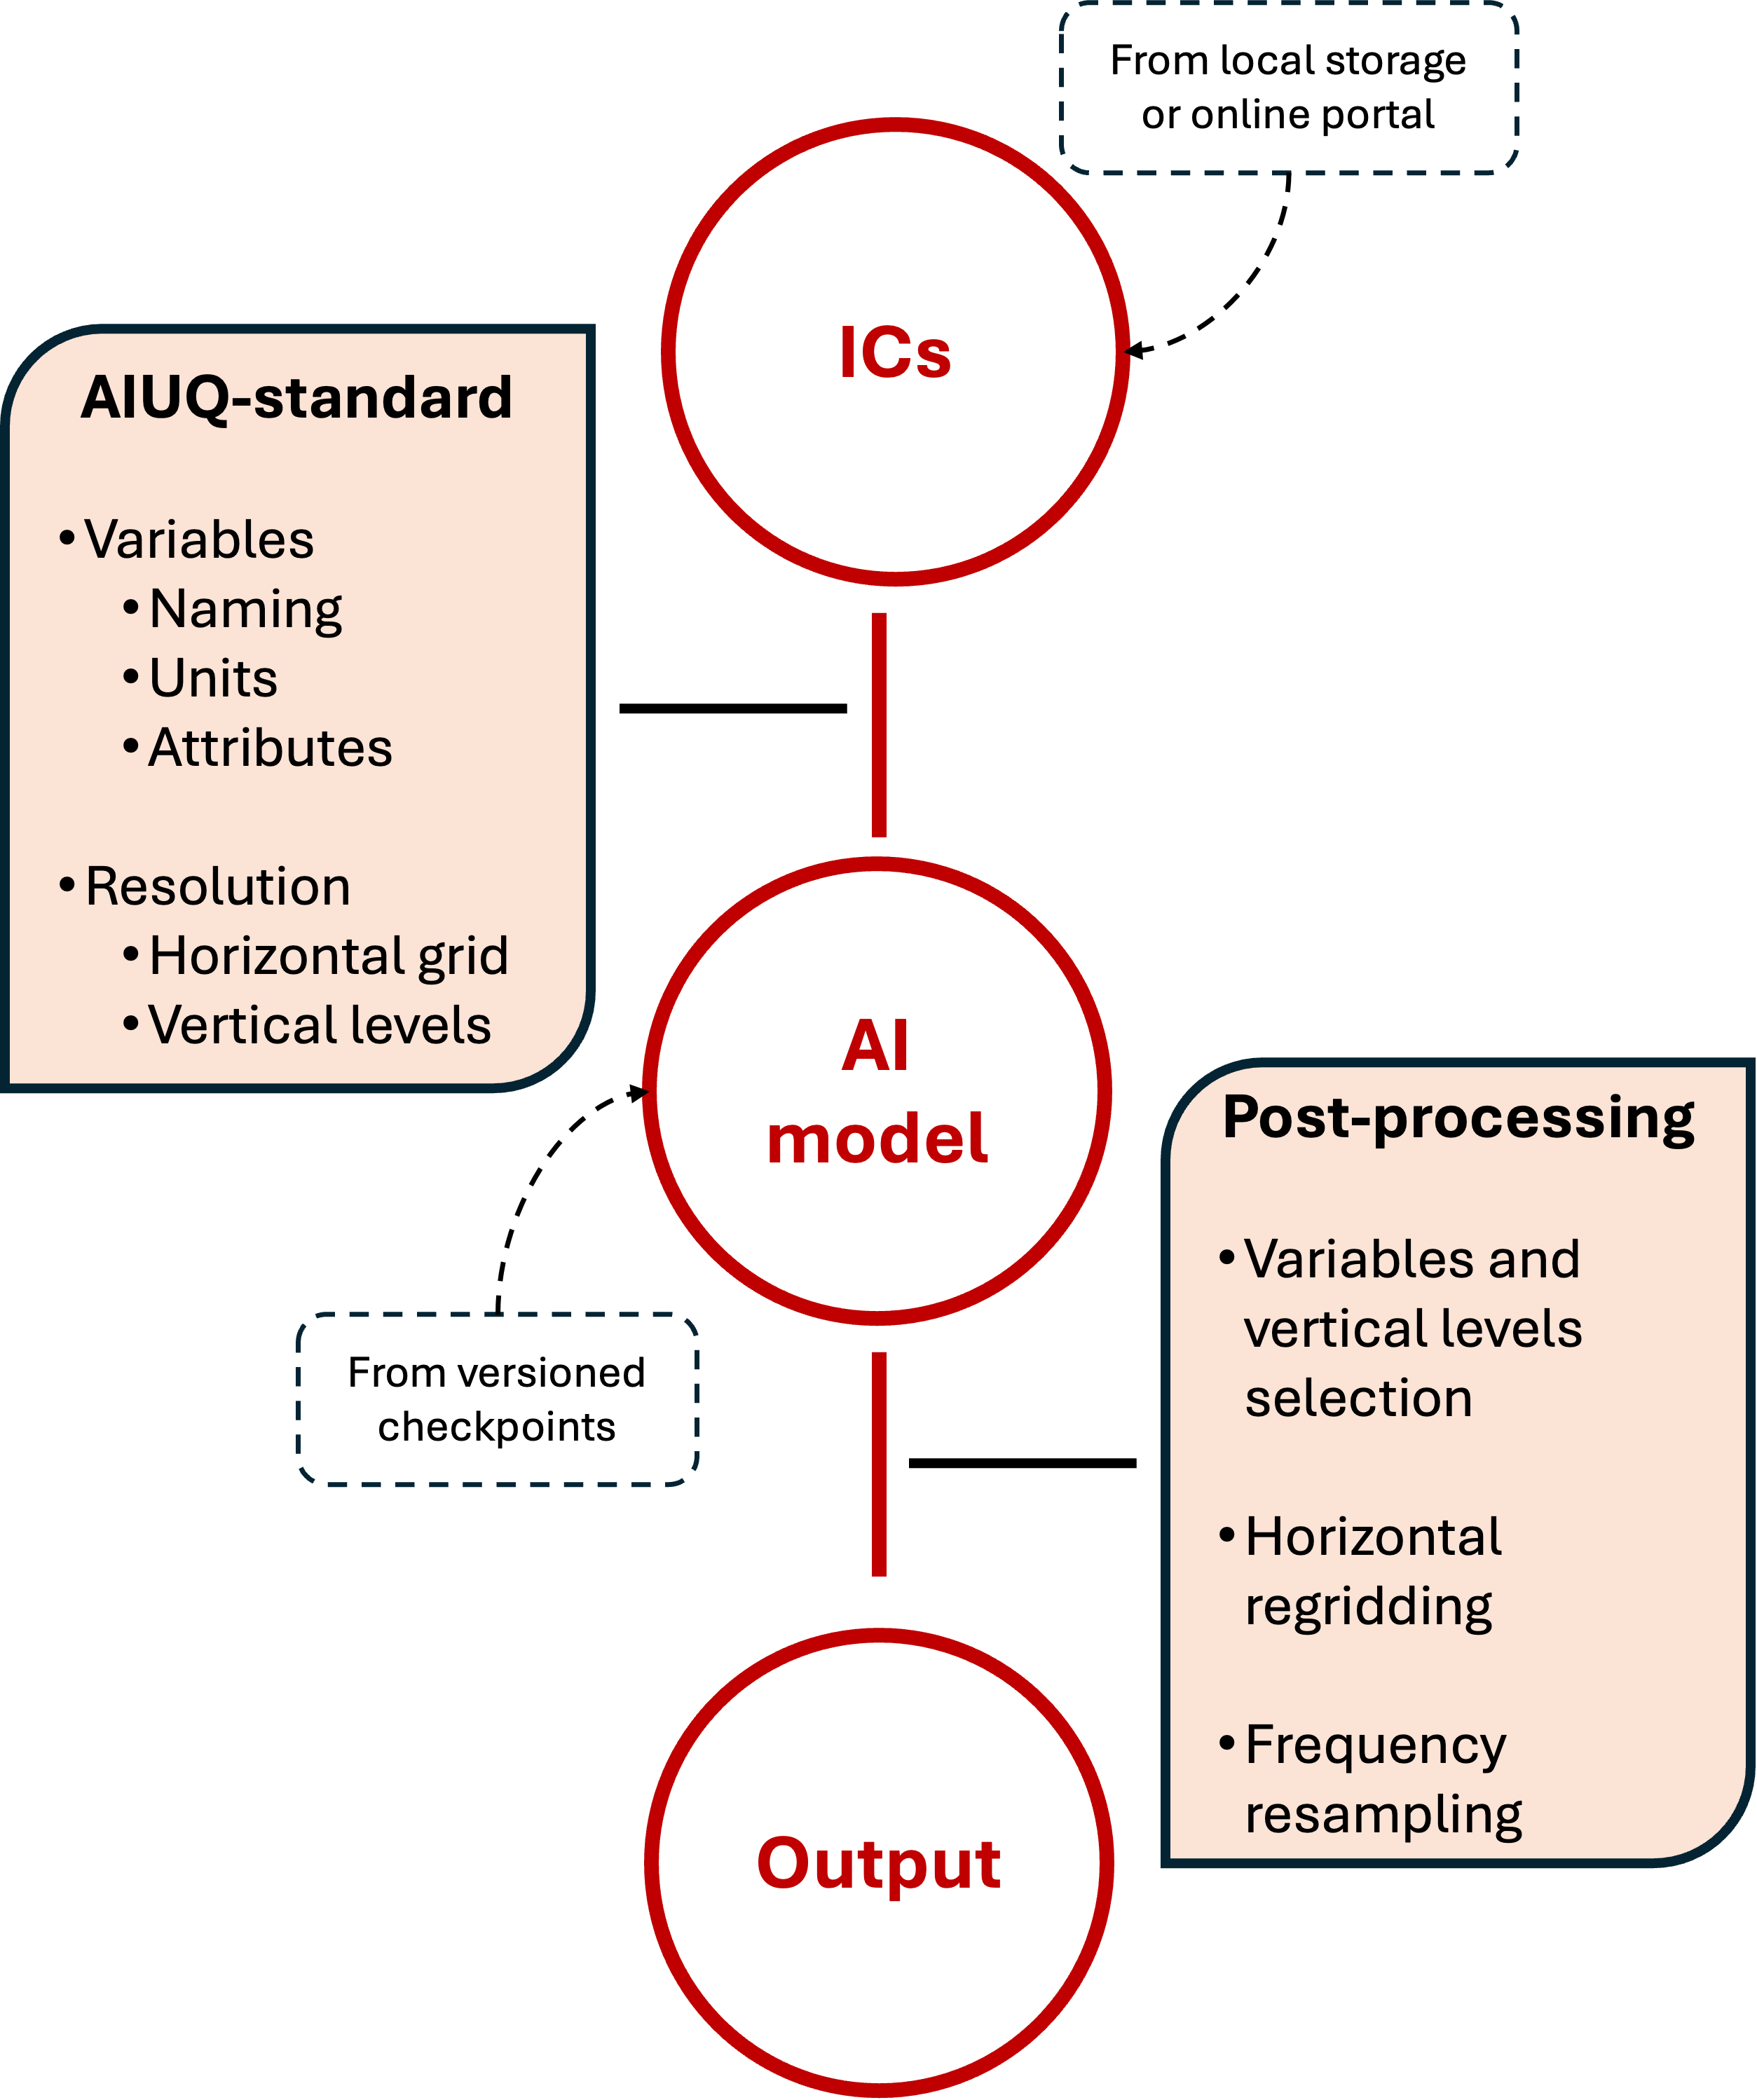
\includegraphics[width=0.55\linewidth]{Chapter2/Figs/aiuq-pipeline.png}
    \caption{Overview of the AIUQ workflow. Source-specific adapters retrieve or read ICs and normalize them to the AIUQ standard. Model-specific adapters translate this common representation to the requirements of the selected checkpoint, while the post-processing stage harmonizes the requested forecast outputs.}
    \label{fig:aiuq-pipeline}
\end{figure}

\paragraph{Configuration} \label{configuration}

An AIUQ experiment is defined declaratively through YAML configuration files. The user selects the forecasting model and checkpoint, the IC source, the initialization dates, the ensemble members, and the temporal chunking of the simulation. The same configuration also describes the requested output variables, pressure levels, temporal frequency, and horizontal resolution. Platform-specific options specify where each task is executed and which computational resources it requires, together with the paths to auxiliary files needed for the execution. At submission time, Autosubmit constructs the experiment graph, combining the specific jobs for the retrieval and preparation of the ICs and for running the inference with the AI models.  

\paragraph{ICs preparation} \label{ics-preparation}

The ICs preparation stage converts heterogeneous input data into a source independent representation. A source adapter either retrieves the requested fields from an online archive or reads them from local storage. Each source is described by an IC card containing its variable names, identifiers, vertical coordinates, and access-specific metadata. These entries are matched against the selected version of the AIUQ standard, after which the retrieved dataset is subset, renamed, and assigned the common coordinates and attributes. Pressure levels and horizontal coordinates are harmonized when necessary. If the primary source does not provide all fields required by the standard, AIUQ invokes the configured fallback hierarchy. 

\paragraph{Fallbacks} \label{fallbacks}
An IC source may not provide every field defined by the AIUQ standard. During IC preparation, AIUQ compares the variable identifiers declared in the source card with those required by the selected standard version. To fill the gaps AIUQ applies a deterministic fallback hierarchy. Missing time-invariant surface fields are first obtained from a shared static dataset; these include orography, the land--sea mask, and descriptors of sub-grid-scale orography obtained from ECMWF. Fields that remain unavailable can then be supplied from a climatological dataset obtained from ERA5. 

\paragraph{Model inference} \label{model-inference}

At the inference stage, the model chosen in the configuration is fed with the ICs prepared at the stage before. A model card maps AIUQ standard to the specific input expected by the model. The adapter then performs only the transformations intrinsic to that backend, such as selecting fields, interpolating to the model grid, changing array layout, or constructing the model's native input state. Inference is executed inside a model-specific container using a versioned checkpoint stored outside the workflow repository. For stochastic models, the ensemble member identifier is also used to initialize the model, making individual realizations reproducible. Model states can be checkpointed where supported, so long integrations such as climate scale simulations can be divided into manageable segments and resumed after interruptions.

\paragraph{Post-processing} \label{post-processing}

The final stage transforms native forecasts into standardized output. AIUQ retains only the variables and vertical levels requested by the user, translates model specific names back to the common convention, and applies the selected temporal aggregation and horizontal regridding. This design avoids storing the full native output when only a subset is needed and makes the computational and storage cost of an experiment configurable. Processed fields are written as NetCDF files organized by variable, ensemble member, and forecast interval, with consistent temporal and spatial coordinates. The resulting simulations therefore share a predictable layout across models and IC sources and can be compared directly or passed to downstream components.


\subsection{Experiment configuration} \label{experiment-configuration}

This study uses ERA5 and the EERIE-AMIP simulations, both representing historical climate conditions. ERA5 \citep{hersbach_era5_2020} is a widely used global reanalysis that combines historical observations with a numerical weather prediction model through data assimilation, providing a reconstruction of past atmospheric conditions. The dataset currently covers the period from 1940 to the present \citep{soci_era5_2024}. ERA5 is extensively used to train AI weather models and serves as a common reference for evaluating their forecasts. Initializing and verifying these models against ERA5 therefore provides a reference configuration closely aligned with their training data in terms of data source. We regard this as an approximately in-distribution setting, without assuming that the training and evaluation distributions are identical. ERA5 fields were retrieved from the public Analysis-Ready, Cloud-Optimized (ARCO) archive hosted on Google Cloud Storage \citep{carver_arco-era5_2023}.

The EERIE-AMIP simulations \citep{aengenheyster_multi-decadal_2026} were produced at ECMWF using an atmosphere-only configuration of the Integrated Forecasting System (IFS), covering 1980--2023. Initialized from ERA5 in January 1980, the simulations evolve freely without atmospheric data assimilation, with prescribed sea surface temperatures, sea ice concentrations, and external radiative forcings. They therefore generate their own weather trajectories rather than reconstructing the observed sequence of weather events. Their climatology is expected to broadly resemble the observed historical climate, although systematic model biases remain. Although ERA5 and EERIE-AMIP both use the IFS, they differ in model configuration and observational constraints. Initializing and verifying AI forecasts against EERIE-AMIP thus provides a potentially out-of-distribution setting, testing generalization to model-generated atmospheric states under broadly comparable historical climate conditions. EERIE-AMIP fields were retrieved through ECMWF's Meteorological Archival and Retrieval System (MARS).

We used two AI-based global weather forecasting models, NeuralGCM and AIFS-CRPS. NeuralGCM \citep{kochkov_neural_2024} combines a differentiable atmospheric dynamical core with neural networks that represent unresolved physical processes, such as cloud formation, radiation, and convection. The model is trained end-to-end on ERA5 trajectories and supports both deterministic and stochastic configurations. In the stochastic configuration, spatially and temporally correlated noise is incorporated into the learned parameterizations, enabling ensemble forecasting. In the original evaluation, the stochastic model at approximately $1.4^\circ$ resolution achieved lower ensemble-mean RMSE and CRPS than the operational ECMWF ensemble for most evaluated variables and lead times up to 15 days. Separate deterministic configurations also reproduced key climate statistics in multi-year to multi-decadal simulations with prescribed sea surface temperature and sea ice.

AIFS-CRPS \citep{lang_aifs-crps_2026} is a probabilistic forecasting model developed at ECMWF. Its encoder--processor--decoder architecture combines an attention mechanisms with a transformer processor and advances the atmospheric state in six-hour steps. The model is trained on ERA5, with operational IFS analyses used for additional training of the medium-range configurations. Ensemble members are generated through stochastic noise injected into the network, while an almost fair CRPS training objective jointly rewards forecast accuracy and appropriate ensemble spread. Published evaluations showed improved CRPS relative to the physics-based IFS ensemble for most variables and lead times up to 15 days. Experiments with a lower-resolution configuration also demonstrated competitive skill for weekly anomalies in 46-day forecasts, extending its potential applications to subseasonal prediction.

For both AI models, 10-member ensemble forecasts were initialized every 10 days during 1985--1990 using atmospheric states from EERIE-AMIP member 1, with each forecast extending to 30 days. The full 10 members EERIE-AMIP ensemble and ERA5 were used as comparison datasets. During post-processing, all datasets were regridded to a common regular latitude--longitude grid with a spacing of $1^\circ \times 1^\circ$ and aggregated into daily means. The analysis focused on temperature at 850 hPa.

\subsection{Evaluation criteria}
\label{evaluation}

The evaluation addresses two complementary aspects of model performance: the accuracy of ensemble forecasts in predicting the evolution of individual weather trajectories, and their ability to reproduce the climatological mean fields of the reference datasets. Forecast accuracy is assessed using the Continuous Ranked Probability Score (CRPS), while climatological agreement is evaluated through global mean bias and spatial root mean square error (RMSE). All metrics are calculated on the common verification grid. Spatial averages are weighted on the cosine of the latitude:

\begin{equation}
    w_i = \frac{A_i}{\sum_{j=1}^{N} A_j},
\end{equation}

where $A_i$ is the area of grid cell $i$ and $N$ is the number of grid cells.

\paragraph{Ensemble forecast accuracy}

The CRPS evaluates a predictive distribution against a verifying value \citep{gneiting_strictly_2007}. For a forecast cumulative distribution function $F$ and a reference value $r$, it is defined as
\begin{equation}
    \mathrm{CRPS}(F,r)
    =
    \int_{-\infty}^{+\infty}
    \left[F(x)-H(x-r)\right]^2 \,\mathrm{d}x,
    \label{eq:crps}
\end{equation}
where $H(x-r)$ is the Heaviside step function, equal to zero for $x<r$ and one for $x\geq r$. For an ensemble of $M$ equally weighted members with predicted values $x_1,\ldots,x_M$, the CRPS of the empirical forecast distribution can equivalently be written as
\begin{equation}
    \mathrm{CRPS}(F,r)
    =
    \frac{1}{M}\sum_{k=1}^{M}|x_k-r|
    -
    \frac{1}{2M^2}
    \sum_{k=1}^{M}\sum_{j=1}^{M}|x_k-x_j|.
    \label{eq:crps-ensemble}
\end{equation}
The score accounts for both the location and spread of the forecast distribution. Lower values indicate better performance, and the score has the same physical units as the evaluated variable. For a deterministic forecast, it reduces to the absolute error.

For the EERIE-initialized experiments, the verifying values are taken from the evolving EERIE-AMIP member~1 trajectory, which also supplies the initial conditions. This comparison therefore evaluates the ability of the AI models to predict the subsequent evolution of the source simulation. The CRPS is calculated locally before spatial averaging with the weights $w_i$, and the resulting global scores are averaged across initialization dates at each lead time.

\paragraph{Climatological agreement}

Daily climatologies are constructed for each day of the year over the study period, with forecast values assigned according to their valid date. These climatologies also retain information about forecast lead time, defined as the time elapsed since initialization. At short lead times, the predicted atmospheric states remain closely tied to the initial conditions and therefore to the source dataset. As lead time increases, this influence gradually weakens, and the forecasts increasingly reflect each AI model's own dynamics and systematic tendencies. Retaining the lead-time dimension therefore allows us to examine how the model climatology evolves during the forecast and whether it progressively departs from that of the initialization dataset.

Climatological differences are evaluated using the area-weighted global mean bias and spatial RMSE. The bias indicates whether the model overestimates or underestimates the reference global mean:

$$
\mathrm{Bias}
=
\sum_{i=1}^{N} w_i
\left(\overline{X}^{A}_{i}-\overline{X}^{R}_{i}\right)
$$

The RMSE measures the magnitude of spatial differences, capturing regional errors that may cancel in the global mean:

\begin{equation}
    \mathrm{RMSE}
    =
    \sqrt{
    \sum_{i=1}^{N} w_i
    \left(\overline{X}^{A}_{i}-\overline{X}^{R}_{i}\right)^2
    } 
\end{equation}

\paragraph{Anomaly amplitude}

The amplitude of daily temperature anomalies is examined as an additional diagnostic of model behaviour. Related measures, often referred to as forecast activity, have been used to assess the magnitude of departures from climatology in AI weather forecasts. Monitoring their evolution with lead time is relevant for identifying changes in atmospheric variability, including the damping or artificial amplification of forecast structures \citep{lang_aifs-crps_2026}.

Daily temperature anomalies are calculated relative to each dataset's own day-of-year climatology over 1985--1990, using the forecast valid date to select the corresponding climatological field. For each initialization, their spatial root mean square is calculated as

\begin{equation}
    \mathrm{RMS}(t)
    =
    \sqrt{
        \sum_{i=1}^{N} w_i
        \left[T'_i(t)\right]^2
    }.
    \label{eq:anomaly-rms}
\end{equation}

where $T'(t)$ denotes the daily temperature anomaly and
$\langle \cdot \rangle_{\mathrm{space}}$ denotes spatial averaging over the global domain.

The resulting curves are examined as a function of forecast lead time and compared with EERIE-AMIP over the corresponding dates. This comparison assesses whether the models maintain comparable anomaly amplitudes as the forecasts progress. 


\section{Results}

\subsection{Computational performance and forecast stability}
\label{sec:performance-stability}

The initial assessment examines the computational feasibility of the experiment and the behaviour of the forecasts over the 30-day integration period. Selected forecasts initialized in 1987 illustrate the main features.

Figure~\ref{fig:example-inference-maps} compares the ensemble-mean temperature at 850~hPa from both AI models with the corresponding EERIE-AMIP member~1 field, ten days after initialization. Both models retain the broad geographical distribution of temperature, including the meridional gradient and the main continental thermal contrasts. Their ensemble means are smoother than the individual EERIE-AMIP realization, consistent with averaging members whose weather patterns progressively diverge. Substantial regional differences nevertheless emerge. The bias patterns of the two models are notably similar, with a spatial correlation coefficient of approximately $r=0.85$ in this example.

The global mean temperature provides a complementary view of forecast evolution (Figure~\ref{fig:global-temperature}). For the three initialization dates shown, AIFS-CRPS develops a recurring cooling tendency during the latter part of the integration, beginning around days 15--20. This behaviour is particularly pronounced in summer (Figure~\ref{fig:global-temperature-summer}), suggesting a forecast drift whose magnitude depends on season and lead time. NeuralGCM does not exhibit the same late-stage cooling in these examples, although its global mean temperature frequently exceeds the EERIE-AMIP reference.

Forecast accuracy was assessed using the CRPS, with the evolving EERIE-AMIP member~1 trajectory as the verification reference (Figure~\ref{fig:crps}). A short NeuralGCM experiment initialized and verified against ERA5 is used as control value, since it provides an example of the performances of the AI model against data extracted from the same distribution as the training set. The CRPS generally increases with lead time and approaches a plateau after approximately 10--15 days, suggesting a loss of the initial conditions. Both EERIE-initialized models follow broadly similar curves, close to the ERA5 control. This suggests that the models conserve the same forecast performances when initialized on a different dataset.

Visual inspection also reveals increasingly anomalous AIFS-CRPS structures over complex terrain. In the Himalayan example (Figure~\ref{fig:example-aifs-degenerative}), temperature and geopotential height patterns remain broadly comparable to EERIE-AMIP at day~15. By day~25, tightly packed, closed geopotential height contours develop around the Tibetan Plateau, intensifying further by day~29 alongside growing temperature differences. Similar artefacts beneath elevated terrain at long lead times are documented by ECMWF for AIFS ENS \citep{ecmwf_known_2026}. During AIFS-CRPS development, some experimental configurations also exhibited artificial growth of small-scale geopotential variability, which propagated towards larger scales \citep{lang_aifs-crps_2026}. This identifies a possible contributing mechanism, but does not establish the cause of the anomalies observed here. Moreover, the 850~hPa surface lies below the terrain across much of this region, where pressure-level fields depend on below-ground extrapolation \citep{ecmwf_atmospheric_2019}. This mechanism is likely causing the cooling in the AIFS-CRPS global temperature observed in Figure~\ref{fig:global-temperature}.

Together, the recurrent global cooling and growing regional anomalies limit the suitability of AIFS-CRPS for generating climate data over the full 30-day period. In the version~1.0 configuration examined here, deterioration becomes apparent after approximately 15--20 days. 

From a computational perspective, both models allowed the experiment to be completed within manageable times. For each model, generating one year of initialization dates, with starts every ten days, ten ensemble members per start, and 30-day forecasts, required approximately one hour on MareNostrum5 using ten GPUs in parallel. The corresponding workload required approximately one day on FELIPE, a computing system at Politecnico di Torino equipped with two GPUs. These timings describe the complete set of forecasts initialized within one year, rather than a continuous year-long integration.

\begin{figure}[p]
    \centering

    % Prima riga: una figura centrata
    \begin{subfigure}{0.9\textwidth}
        \centering
        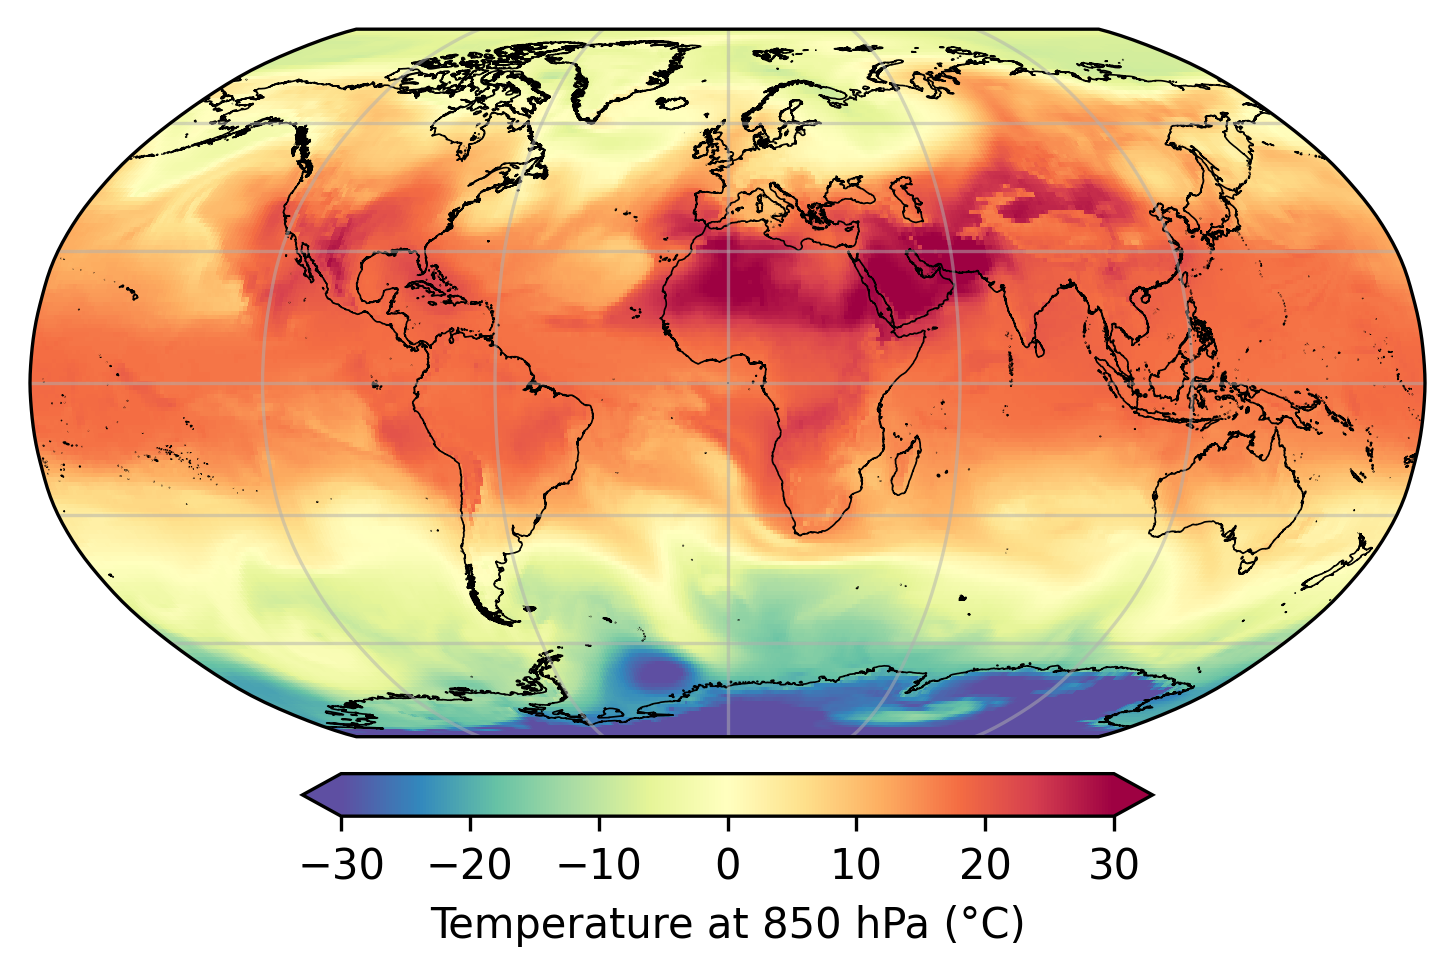
\includegraphics[width=\linewidth]{Chapter2/Figs/eerie_temperature.png}
        \caption{EERIE-AMIP (first member)}
        \label{fig:eerie-esample}
    \end{subfigure}

    \par\medskip

    % Seconda riga: due figure
    \begin{subfigure}{0.49\textwidth}
        \centering
        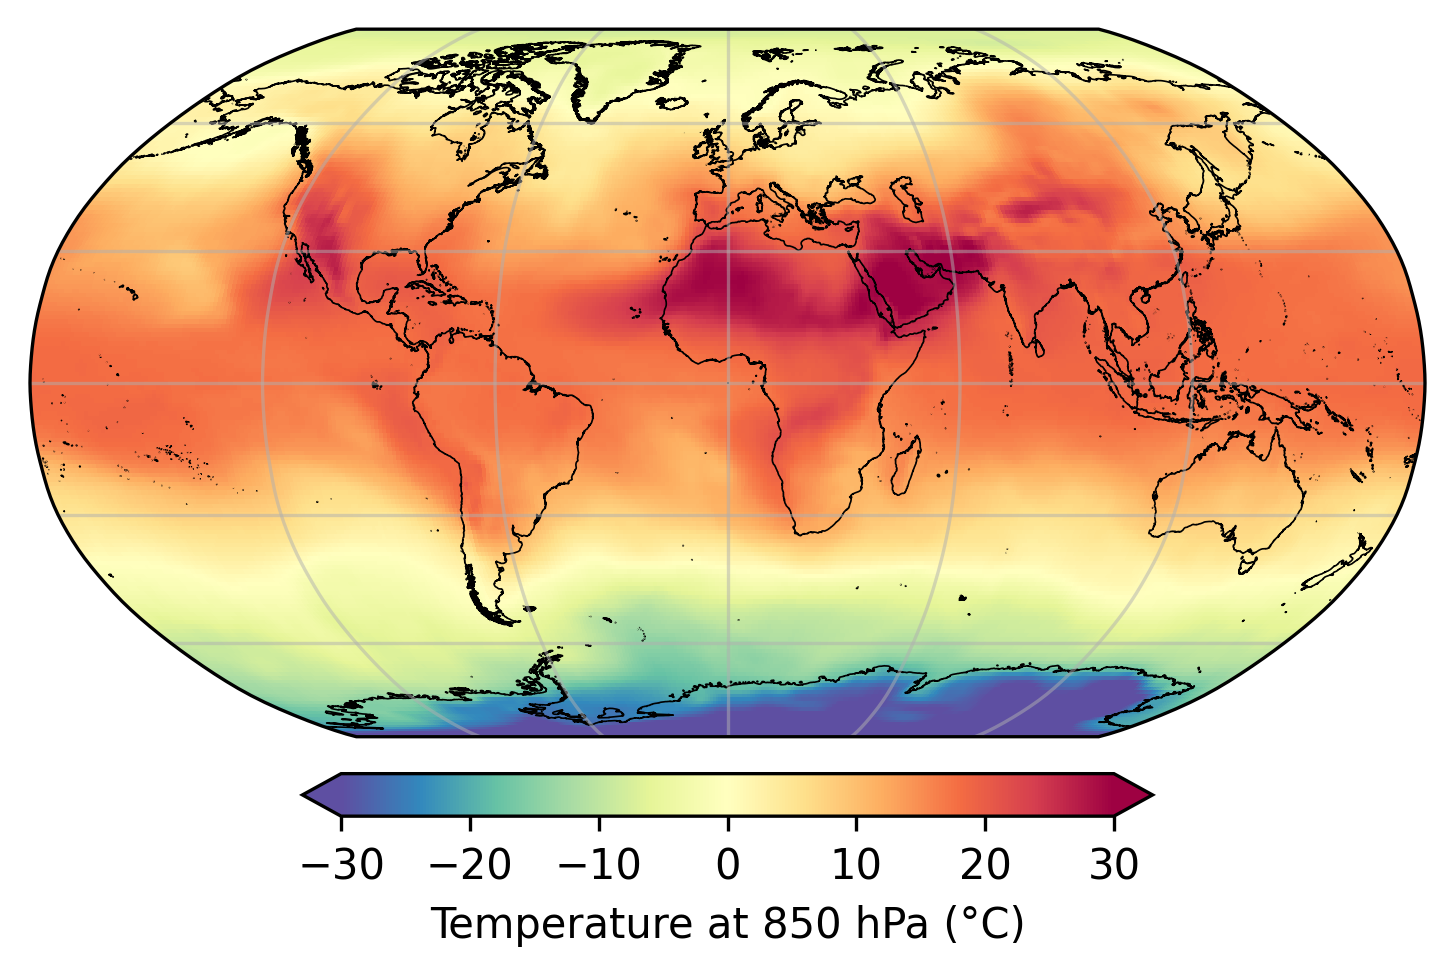
\includegraphics[width=\linewidth]{Chapter2/Figs/ngcm_temperature.png}
        \caption{NeuralGCM ensemble average}
        \label{fig:ngcm-example}
    \end{subfigure}
    \hfill
    \begin{subfigure}{0.49\textwidth}
        \centering
        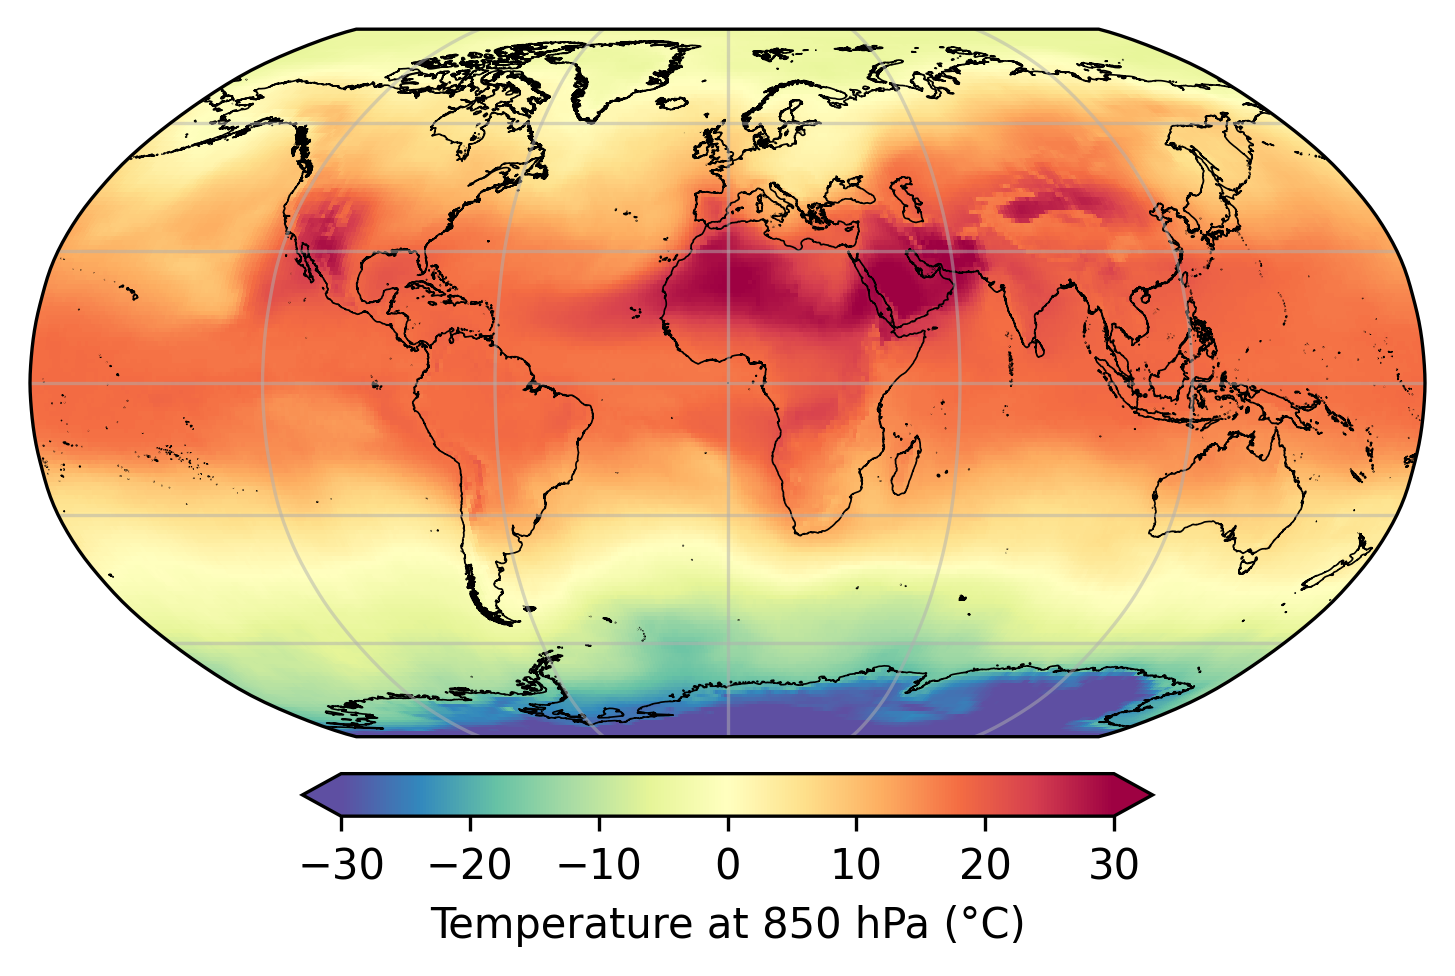
\includegraphics[width=\linewidth]{Chapter2/Figs/aifs_temperature.png}
        \caption{AIFS-CRPS ensemble average}
        \label{fig:aifs-example}
    \end{subfigure}

    \par\medskip

    % Terza riga: due figure
    \begin{subfigure}{0.49\textwidth}
        \centering
        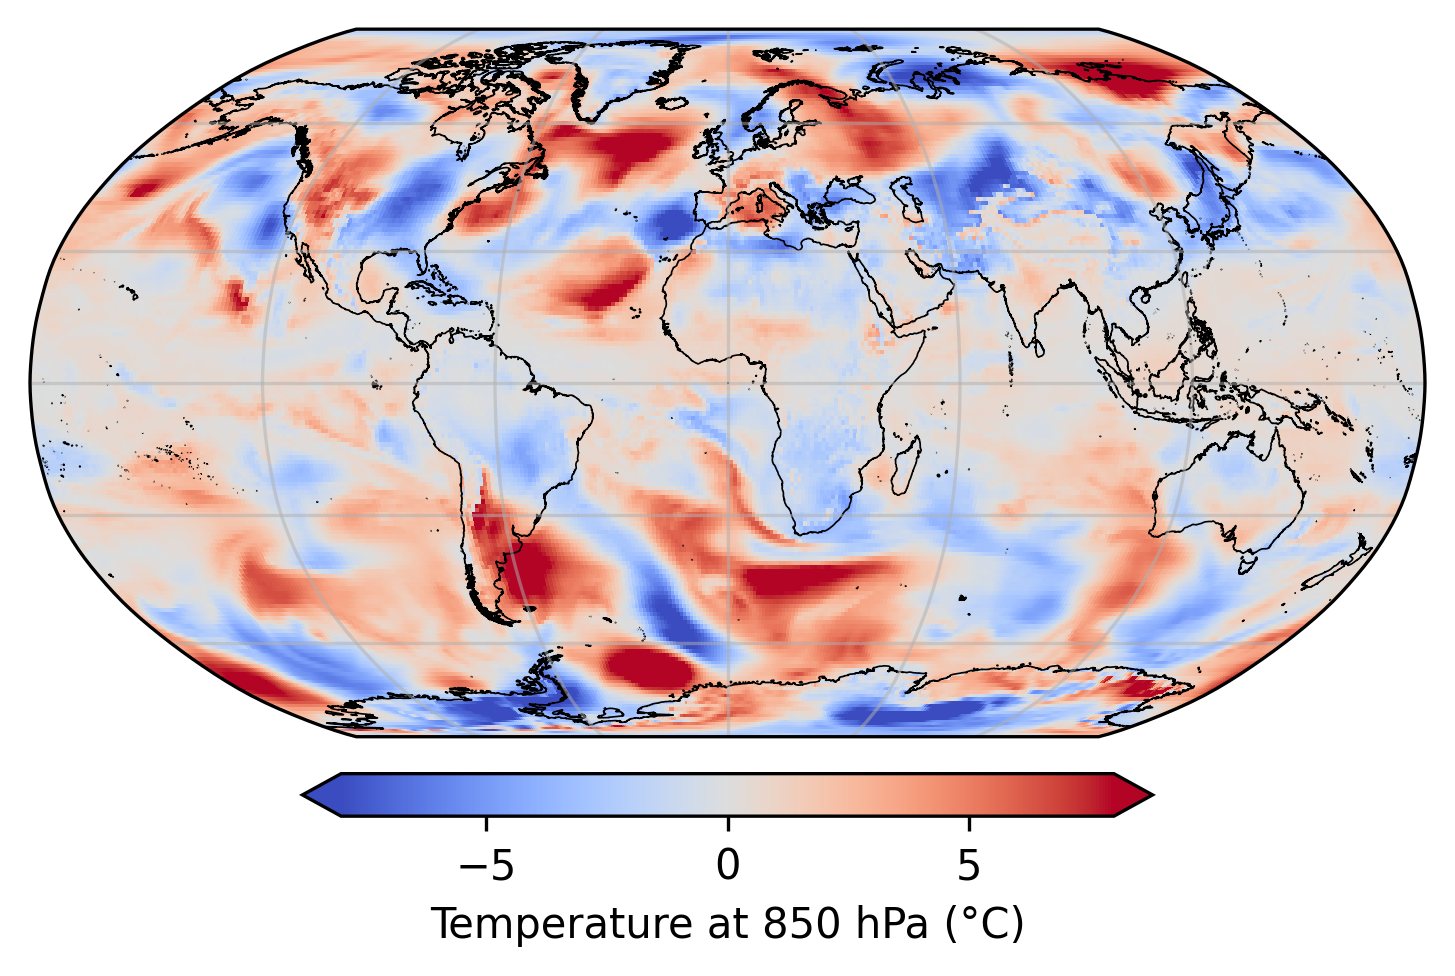
\includegraphics[width=\linewidth]{Chapter2/Figs/ngcm_bias.png}
        \caption{NeuralGCM bias}
        \label{fig:ngcm-bias-example}
    \end{subfigure}
    \hfill
    \begin{subfigure}{0.49\textwidth}
        \centering
        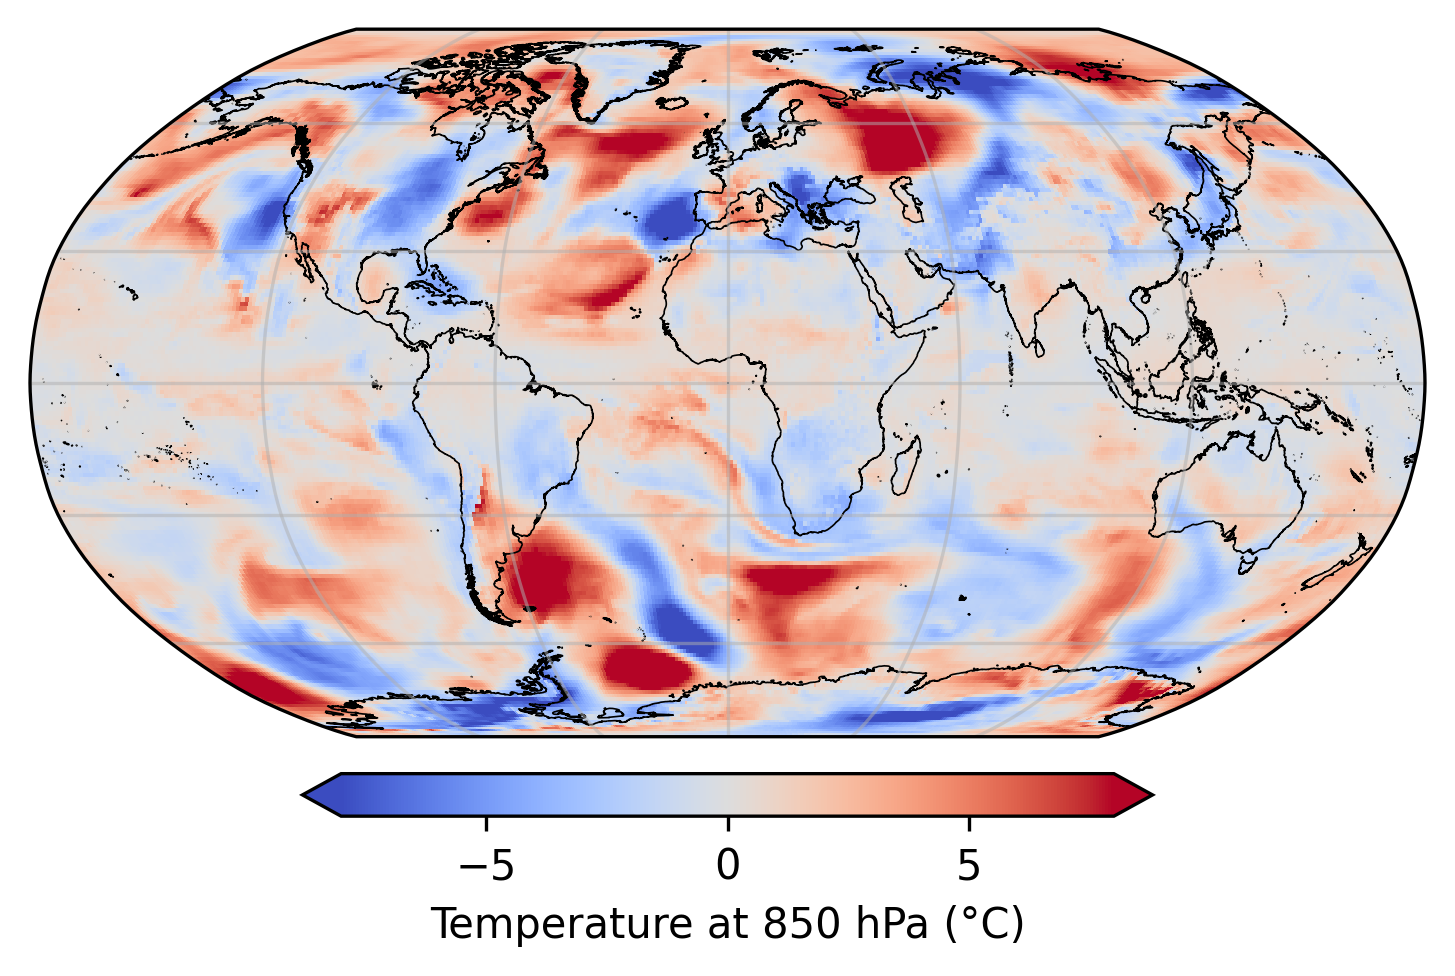
\includegraphics[width=\linewidth]{Chapter2/Figs/aifs_bias.png}
        \caption{AIFS-CRPS bias}
        \label{fig:aifs-bias-example}
    \end{subfigure}

    \caption{Temperature at 850~hPa at a lead time of 10 days for AI forecasts initialized from the EERIE-AMIP first member at June 10th 1987. (a) The verifying EERIE-AMIP member~1 field at the same valid time. (b,c) Ensemble-mean forecasts from NeuralGCM and AIFS-CRPS, respectively, each based on 10 ensemble members. (d,e) Corresponding ensemble-mean temperature differences relative to EERIE-AMIP member~1.}
    \label{fig:example-inference-maps}
    
\end{figure}


\begin{figure}[H]
    \begin{subfigure}{1\textwidth}
        \centering
        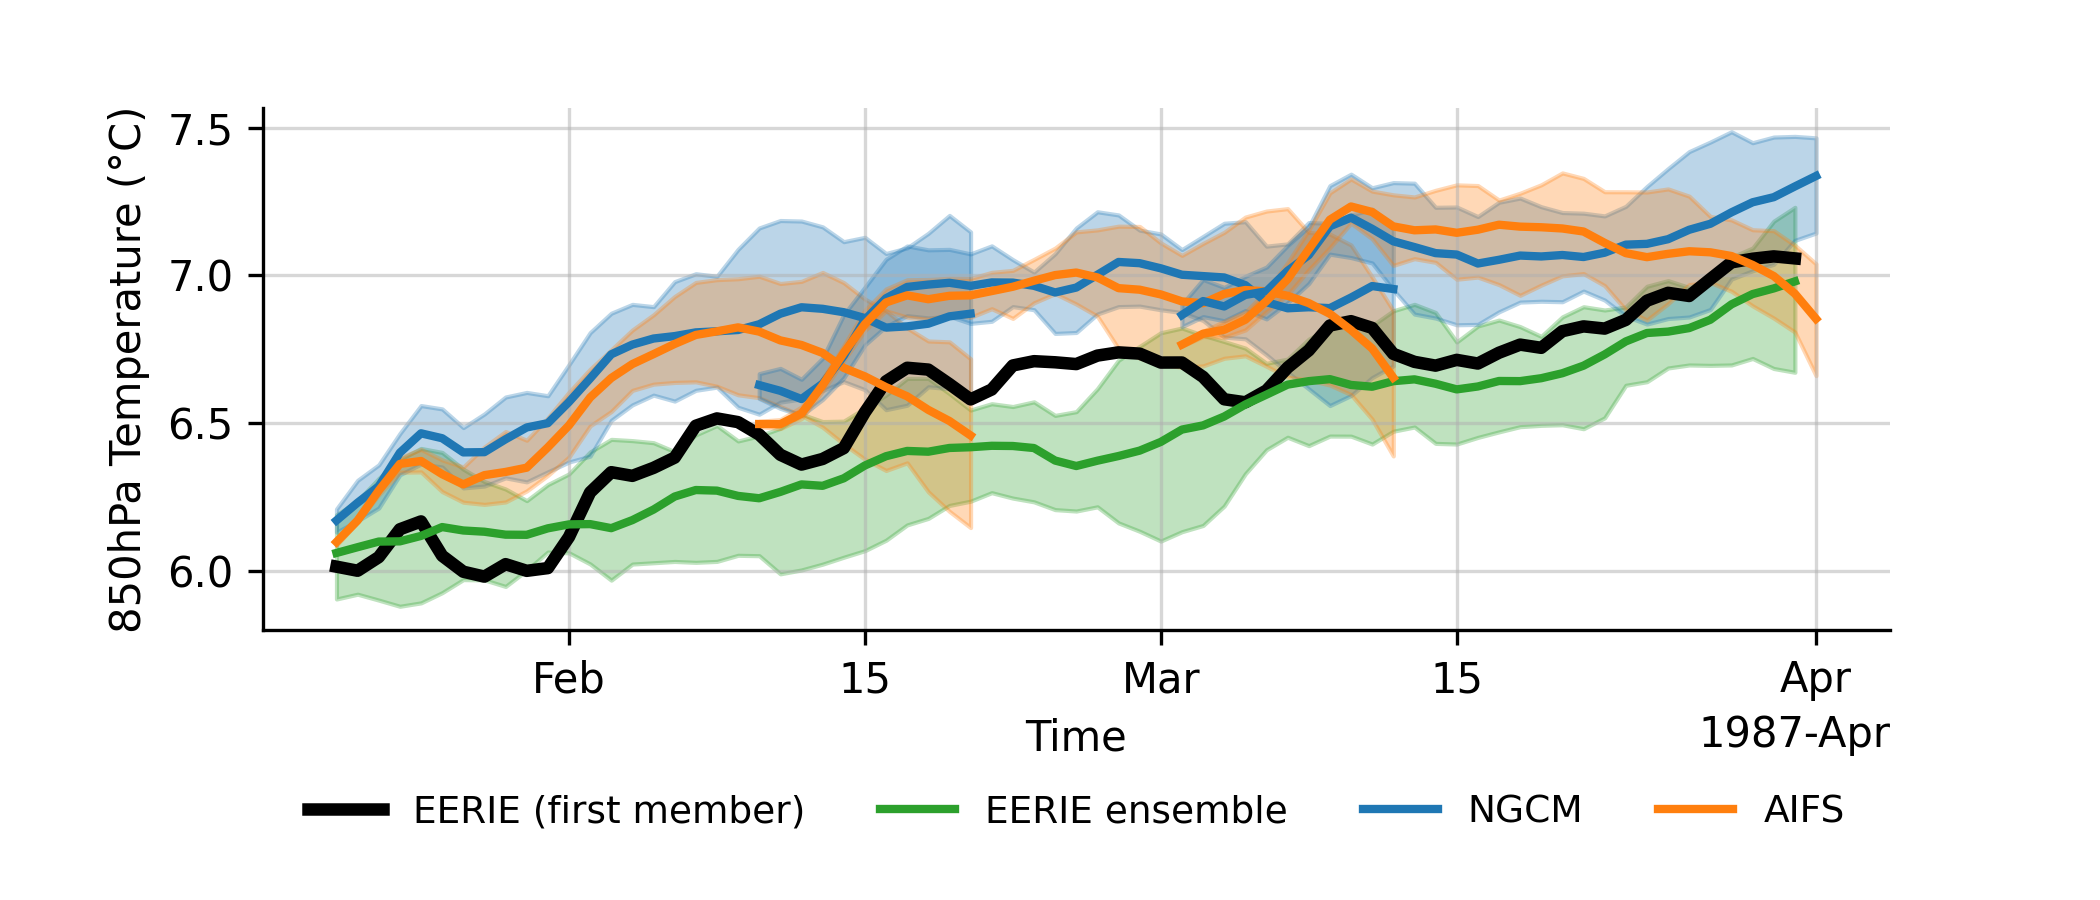
\includegraphics[width=0.8\linewidth]{Chapter2//Figs/cool_lines_plot_winter.png}
        \caption{Winter 1987.}
        \label{fig:global-temperature-winter}
    \end{subfigure}

    \par\medskip

    \begin{subfigure}{1\textwidth}
        \centering
        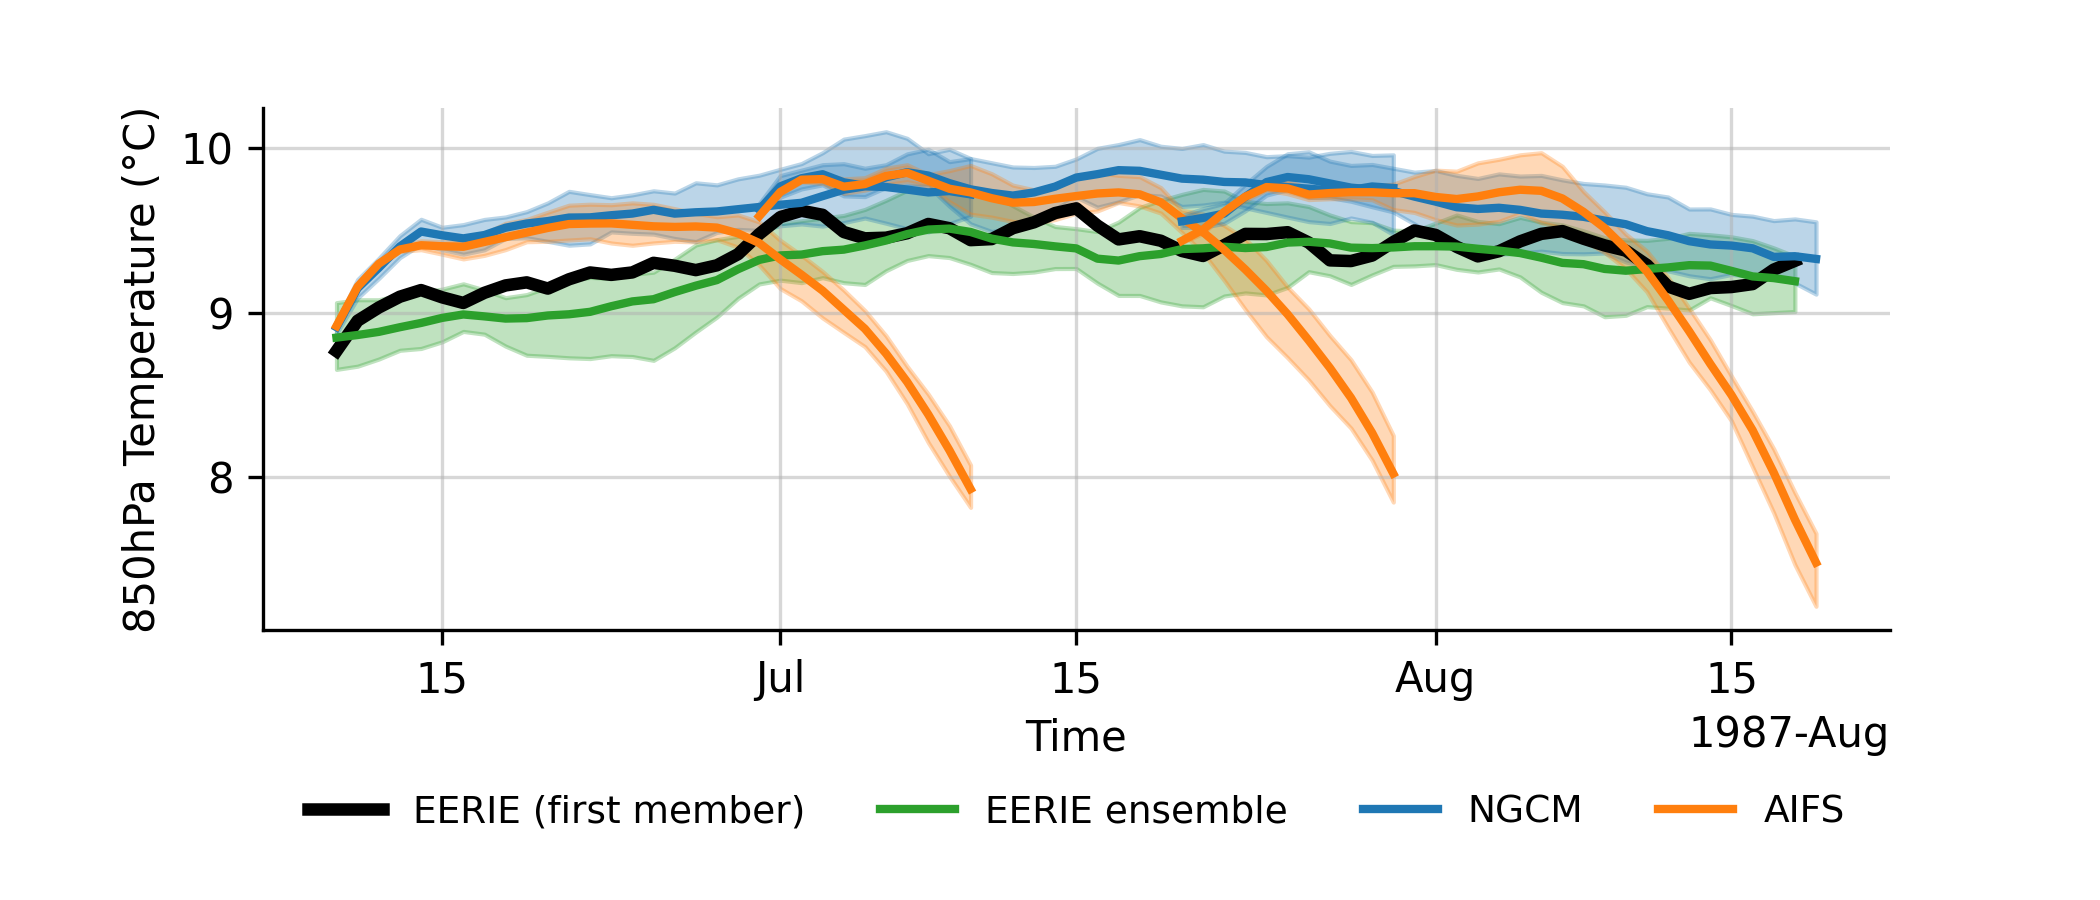
\includegraphics[width=0.8\linewidth]{Chapter2//Figs/cool_lines_plot_summer.png}
        \caption{Summer 1987.}
        \label{fig:global-temperature-summer}
    \end{subfigure}

    \caption{Global mean temperature at 850~hPa. The black line shows EERIE-AMIP member 1, which provides the initial conditions for the AI forecasts, while the green line represents the mean of the remaining nine EERIE-AMIP members. Blue and orange lines show the ensemble means of NeuralGCM and AIFS-CRPS. The forecasts have been initialized on 21 January, 10 February, and 2 March 1987 (panel a) and on June 10, June 30 and July 20 1987 (panel b). Shaded bands indicate the 5th--95th percentile range across the corresponding ensemble members, calculated from their individual global mean temperatures.}
    \label{fig:global-temperature}
    
\end{figure}


\begin{figure}[H]
    \centering
    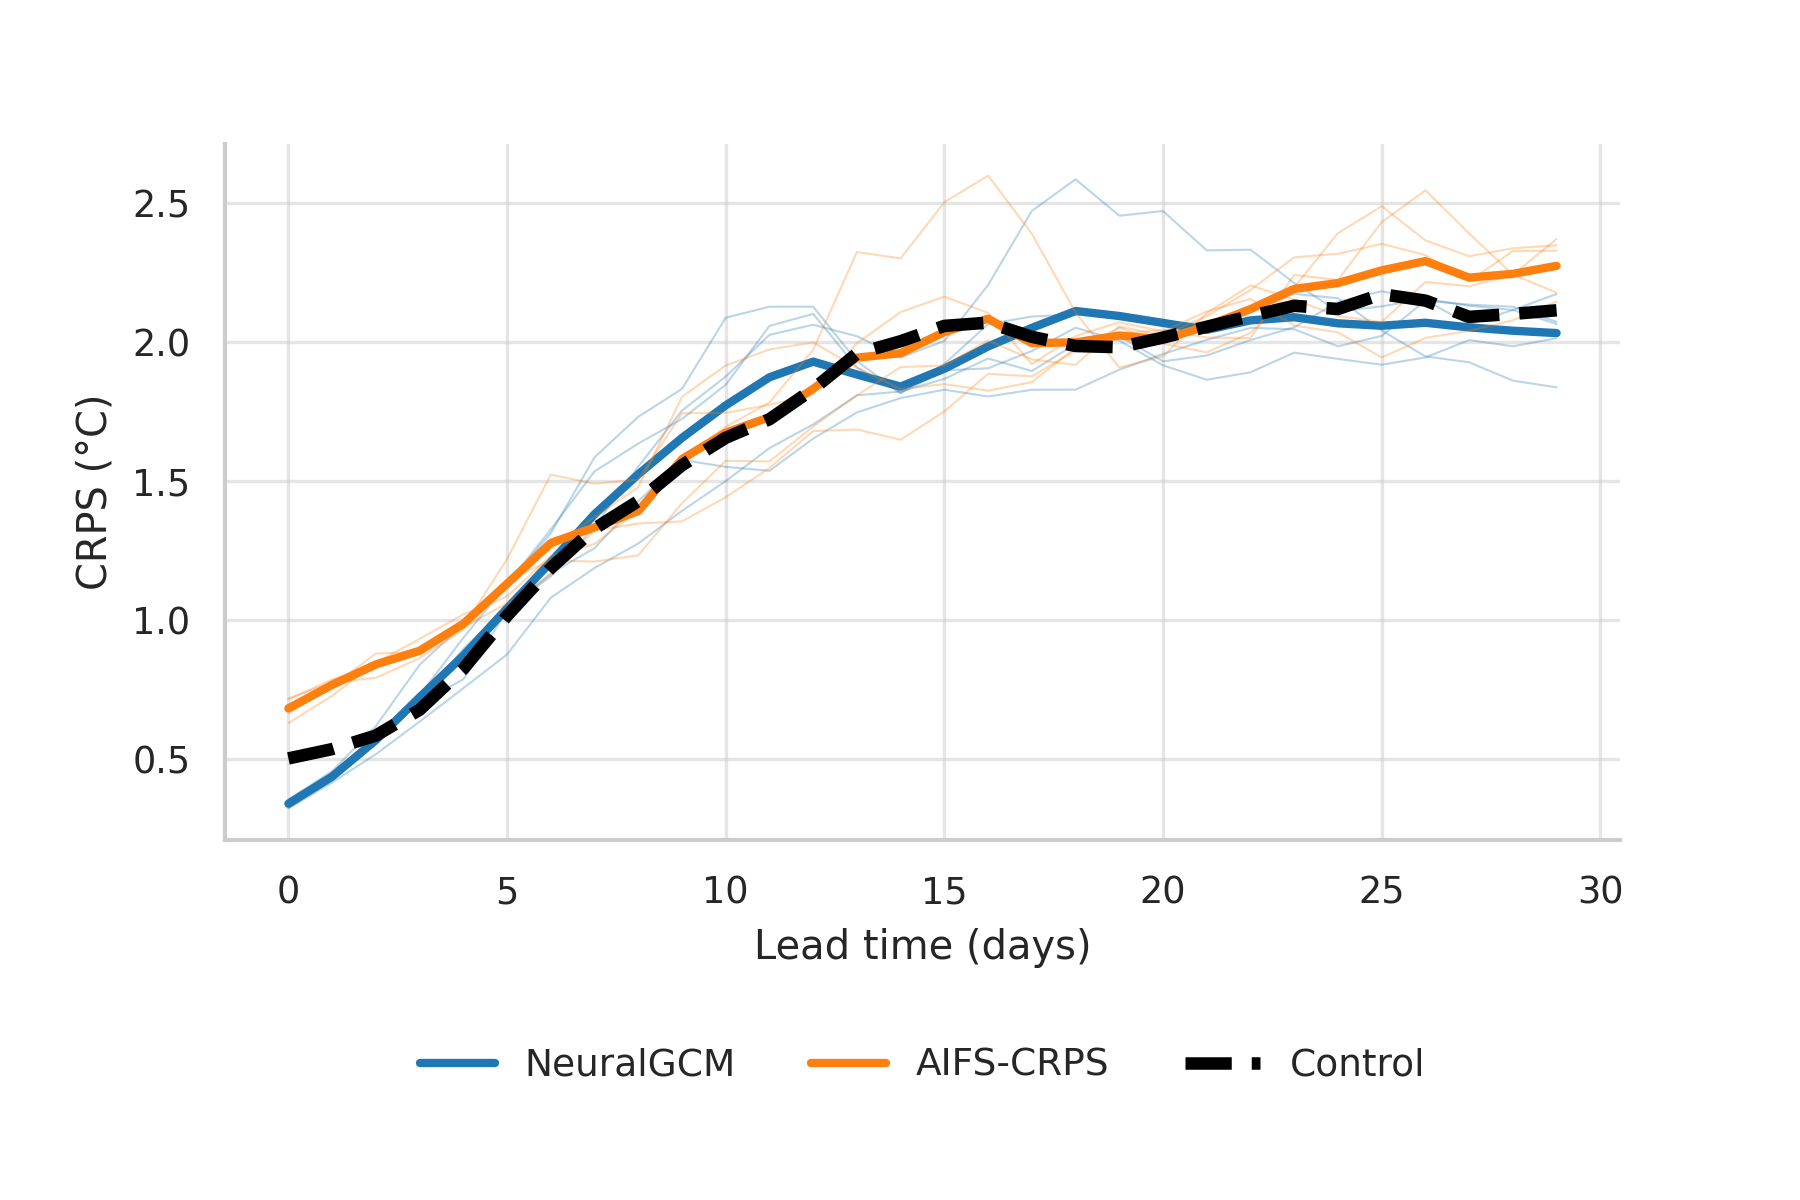
\includegraphics[width=0.75\linewidth]{Chapter2//Figs/crps_global.png}
    \caption{Spatially averaged CRPS of 850 hPa temperature as a function of forecast lead time. NeuralGCM and AIFS ensemble forecasts are verified against the first member of EERIE-AMIP for two randomly selected initialization dates in 1985--1990. Thin lines show the CRPS for each initialization date; thick lines show the mean across the selected EERIE initializations. The dashed black control line shows the mean CRPS of NeuralGCM-ERA against ERA5 across eight initialization dates randomly selected in 1985.}
    \label{fig:crps}
\end{figure}

\begin{figure}[p]
    \centering

    % Prima riga: una figura centrata
    \begin{subfigure}{1\textwidth}
        \centering
        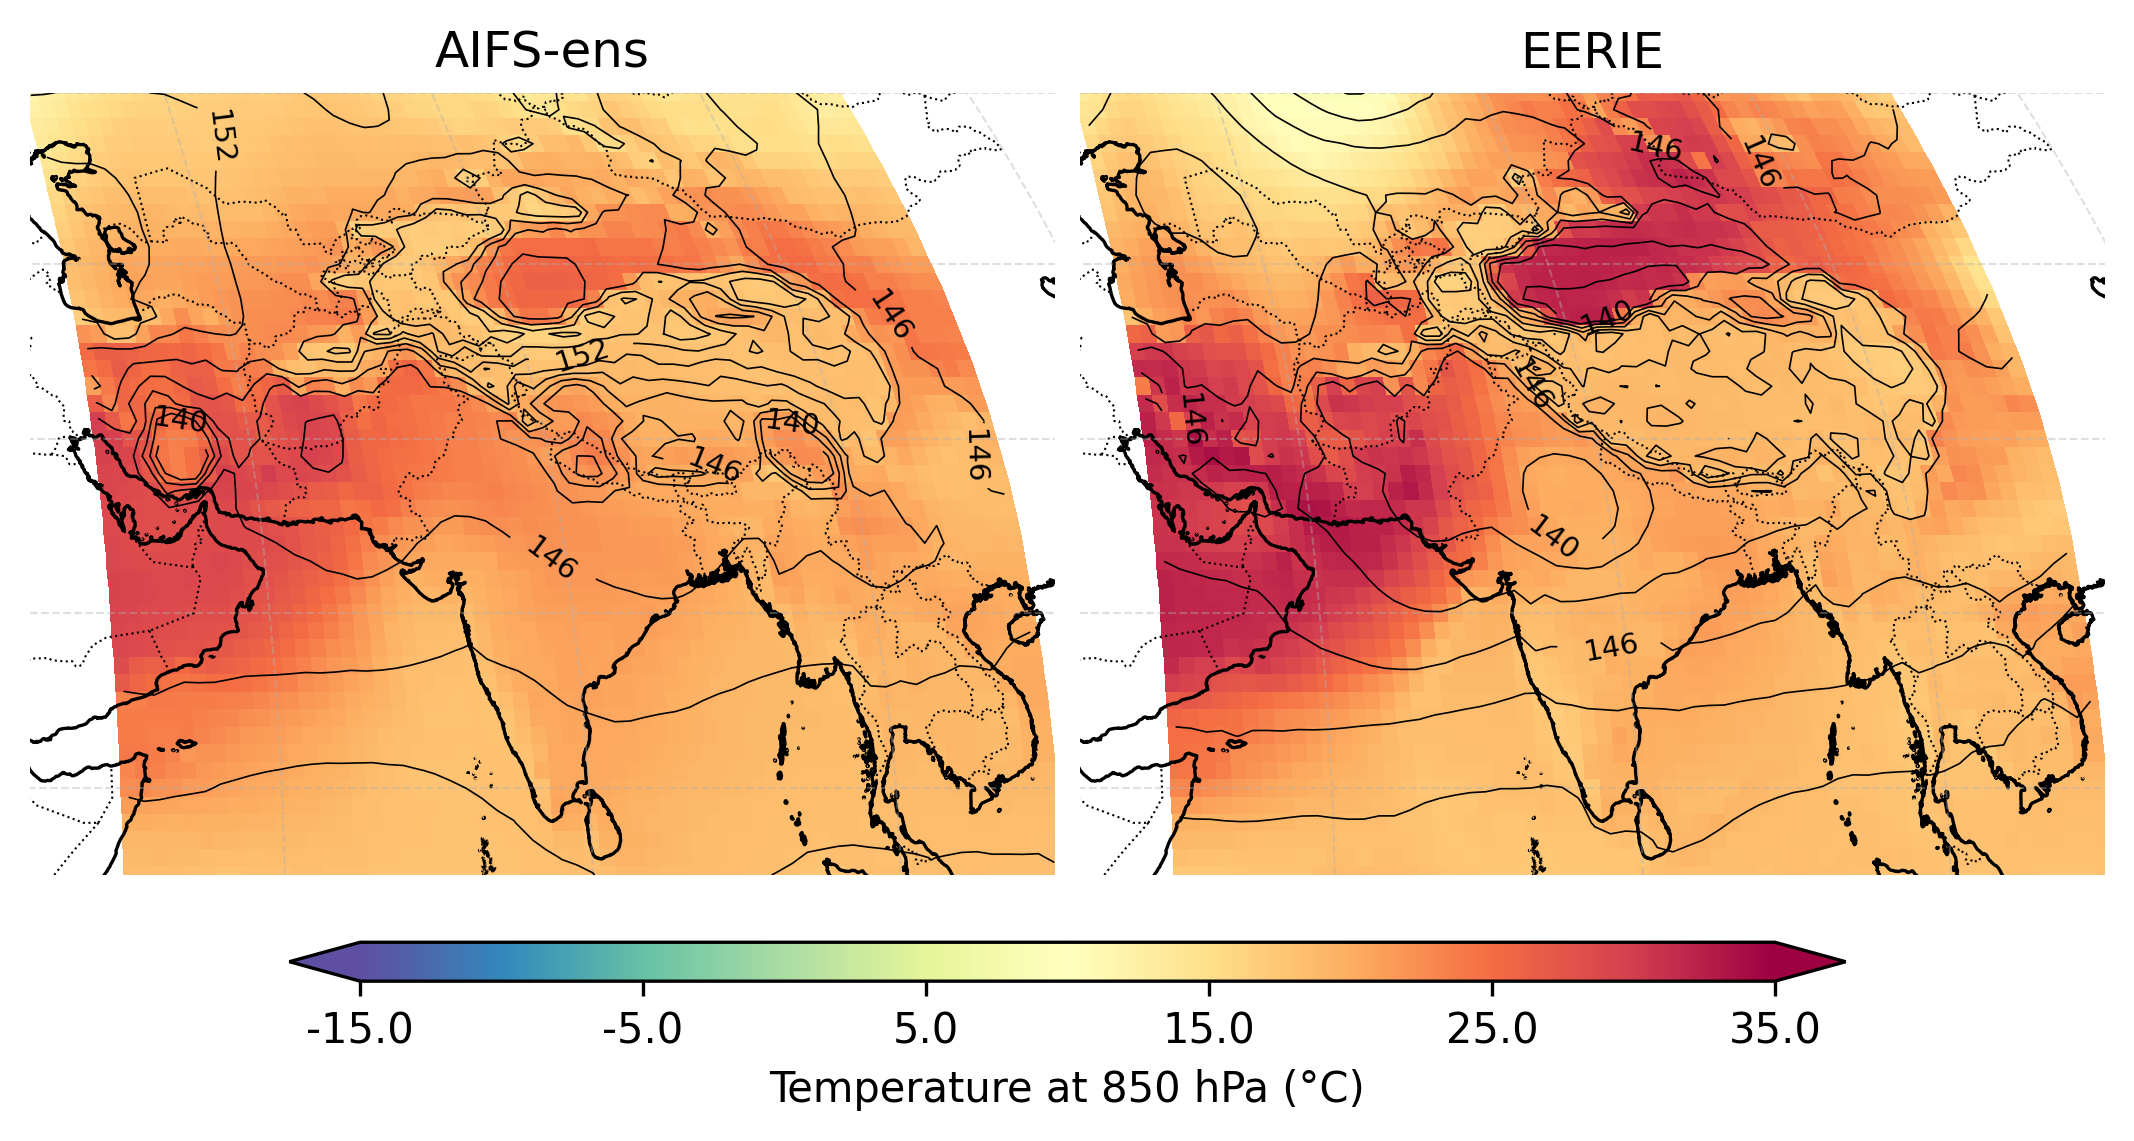
\includegraphics[width=0.6\linewidth]{Chapter2/Figs/comparison_ens_aifs_15_India.png}
        \caption{Lead time: 5 days}
        \label{fig:5-days-india}
    \end{subfigure}

    \par\medskip

    \begin{subfigure}{1\textwidth}
        \centering
        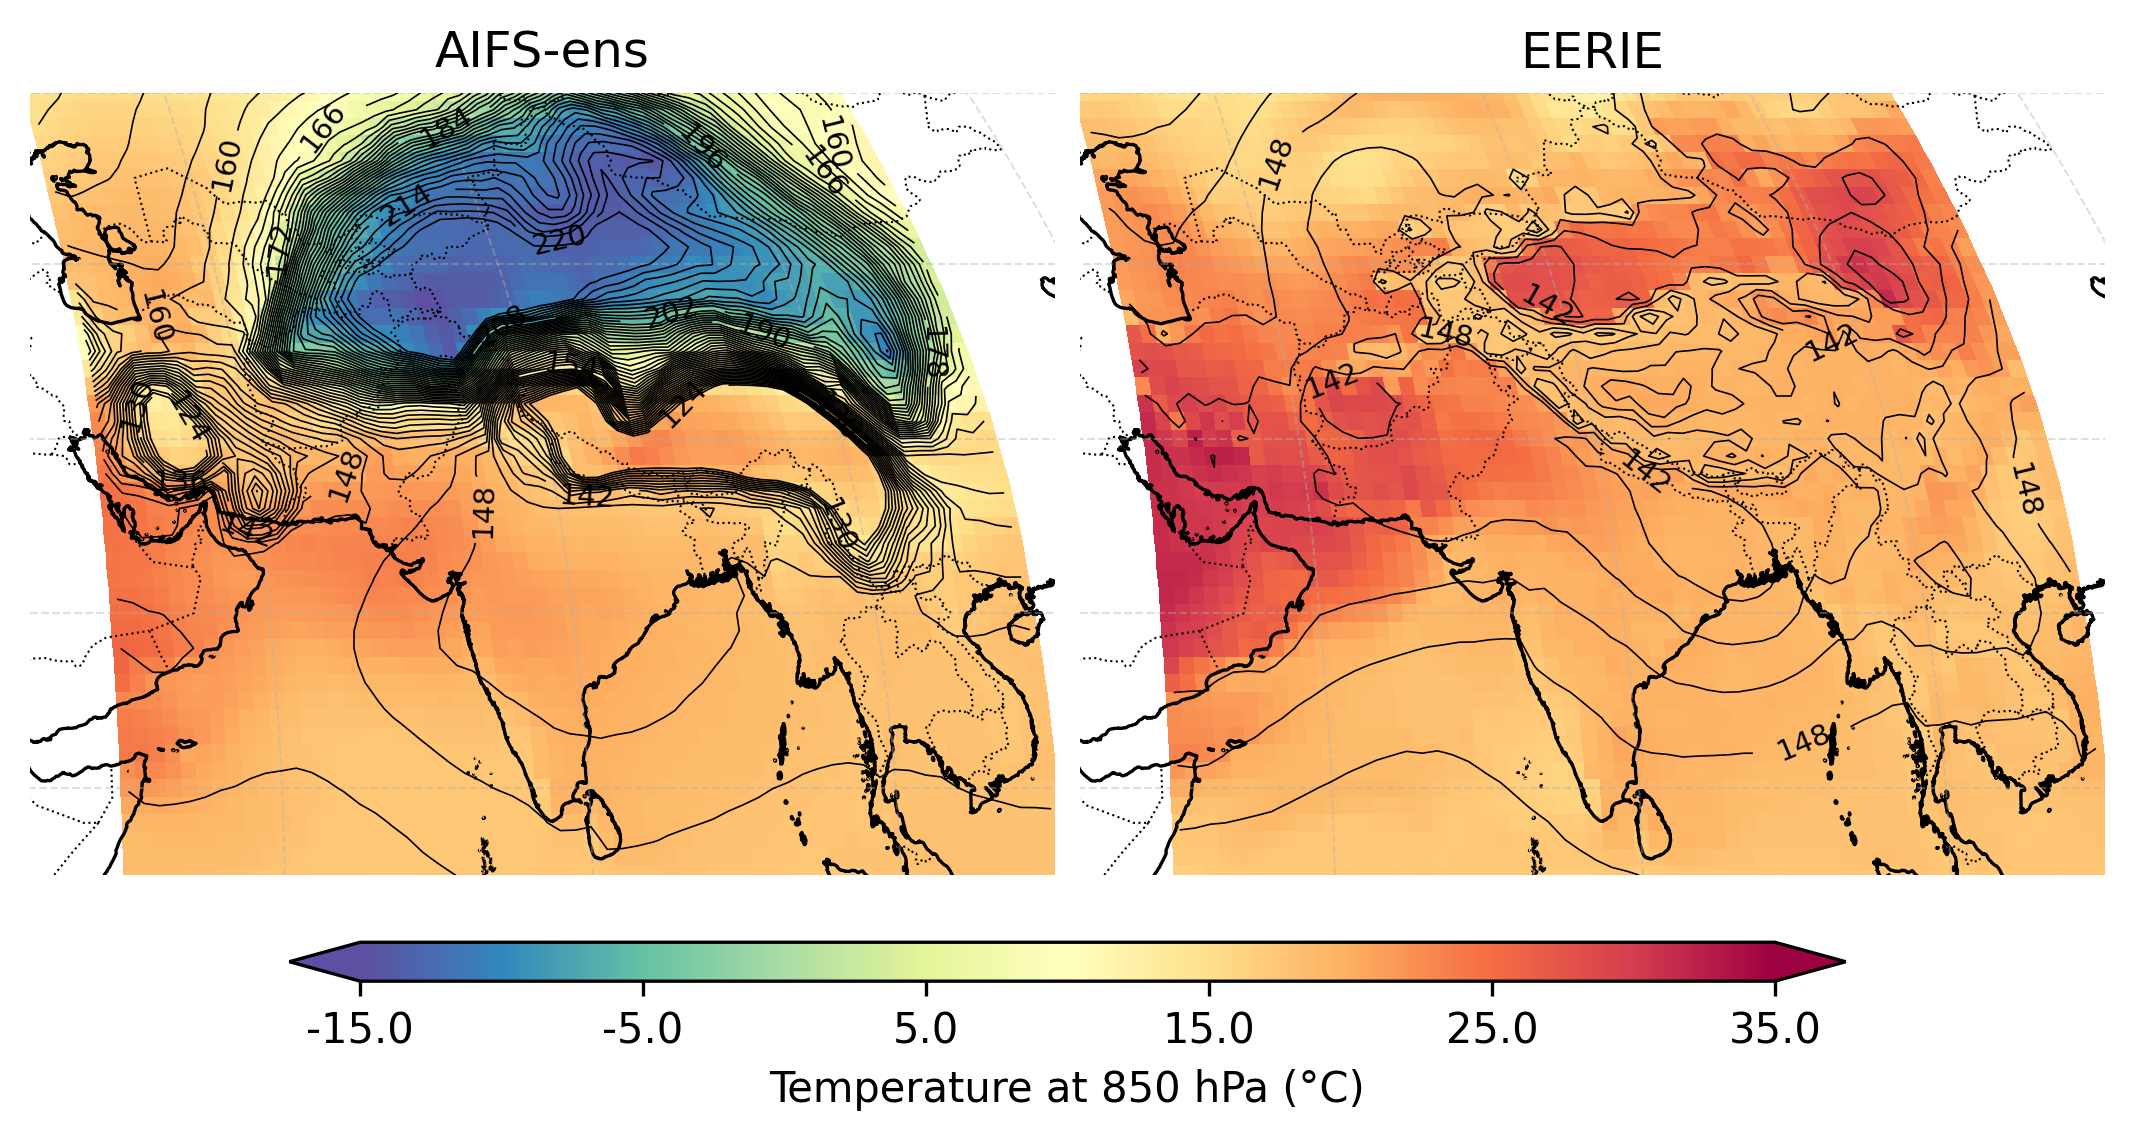
\includegraphics[width=0.6\linewidth]{Chapter2/Figs/comparison_ens_aifs_25_India.png}
        \caption{Lead time: 25 days}
        \label{fig:25-days-india}
    \end{subfigure}


    \par\medskip

    \begin{subfigure}{1\textwidth}
        \centering
        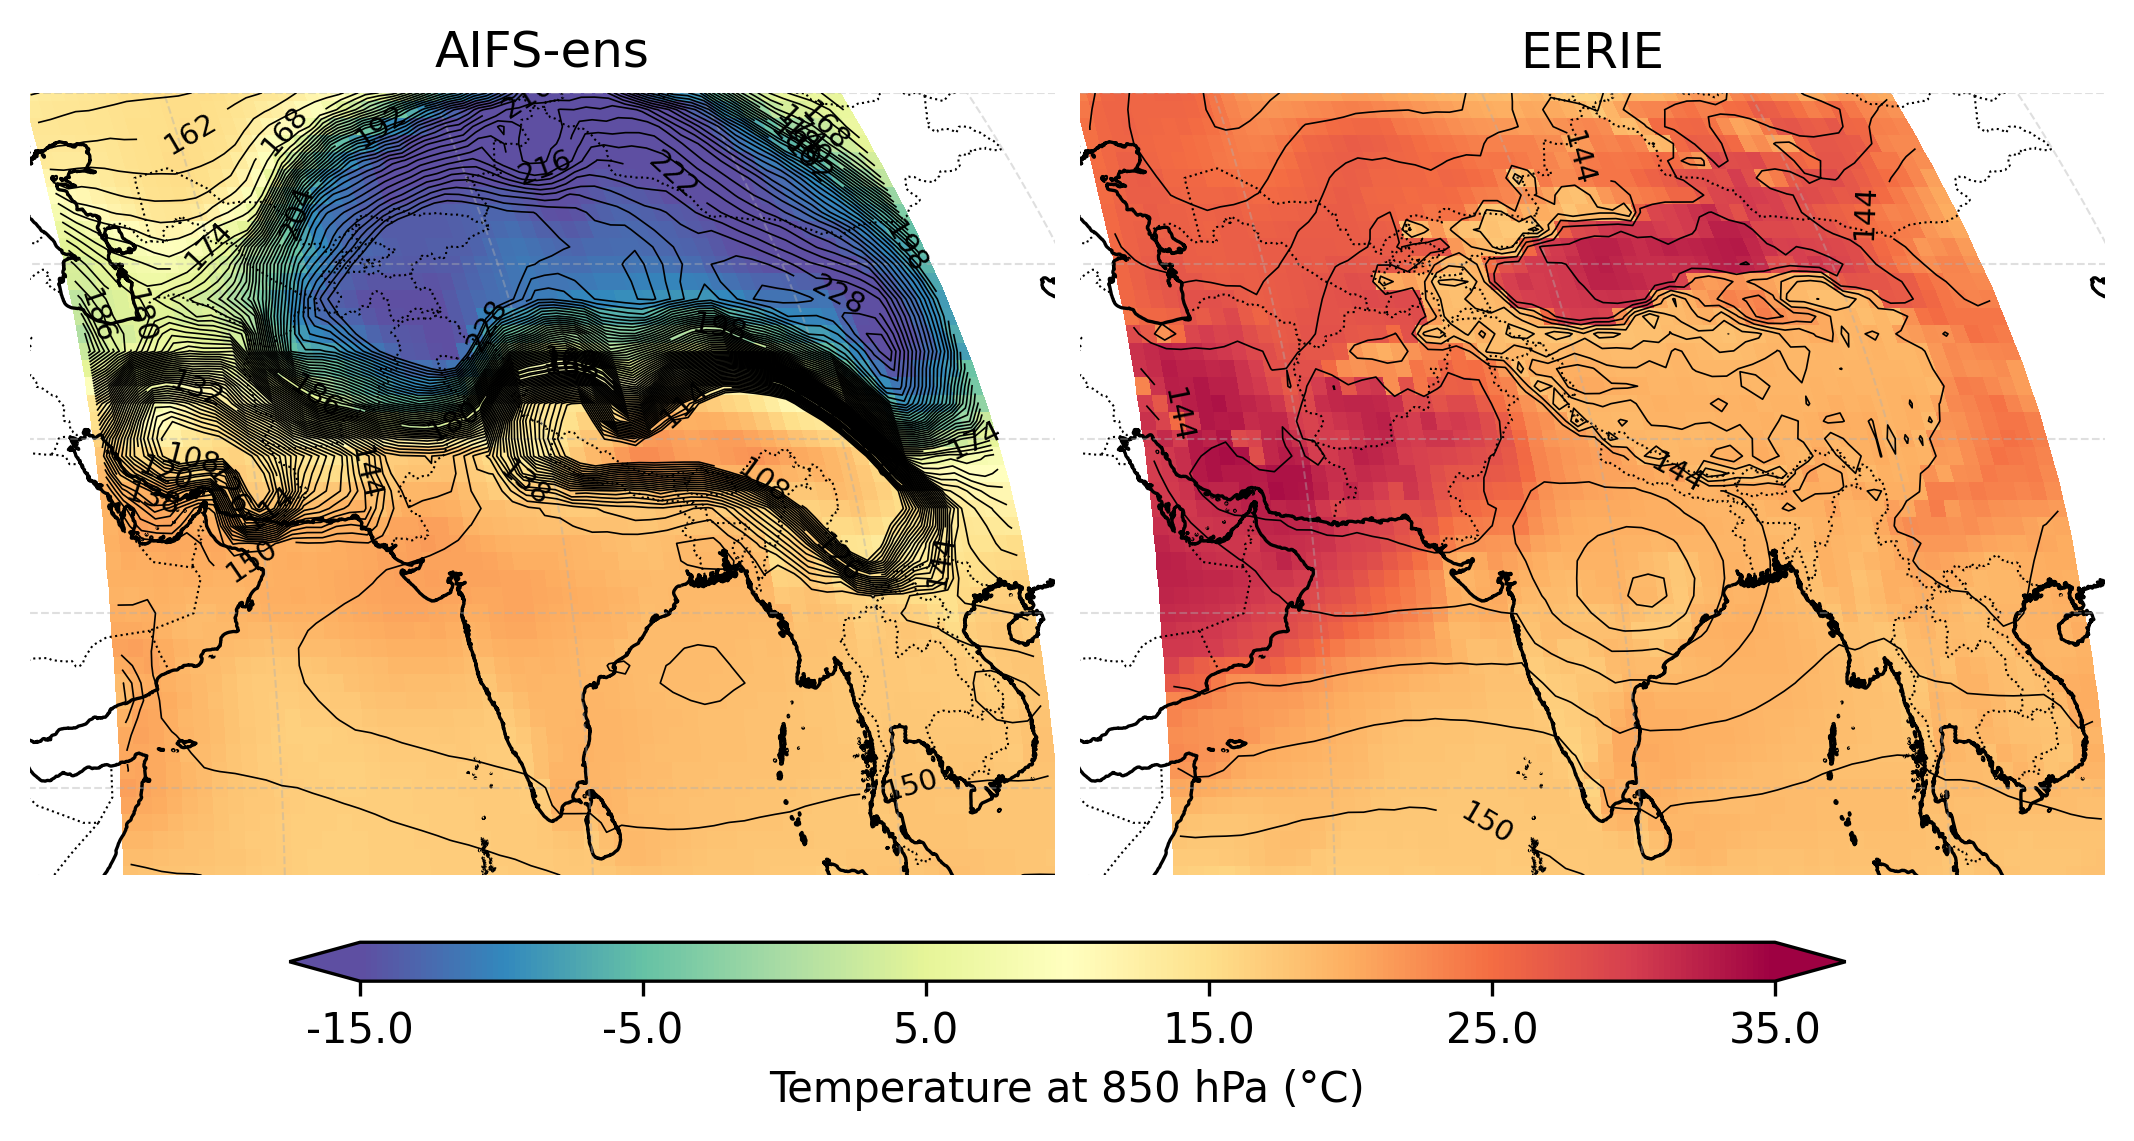
\includegraphics[width=0.6\linewidth]{Chapter2/Figs/comparison_ens_aifs_29_India.png}
        \caption{Lead time: 29 days}
        \label{fig:29-days-india}
    \end{subfigure}

    \caption{Development of an anomalous pattern over the Himalayan region in an AIFS-CRPS forecast initialized on 10 June 1987. Panels show the 10-member ensemble mean at lead times of (a) 15, (b) 25, and (c) 29 days. Shading represents temperature at 850~hPa, while contours indicate geopotential height at the same pressure level, expressed in decametres (dam).}
    \label{fig:example-aifs-degenerative}
\end{figure}

\clearpage

\subsection{AI Model Climatology}

The climatological evaluation examines whether forecasts initialized from EERIE-AMIP preserve the mean climatic conditions of the source simulation as lead time increases. Comparisons with EERIE-AMIP and ERA5 provide complementary information: the former assesses consistency with the initialization dataset, while the latter indicates how closely the generated fields resemble the reanalysis used to train the AI models. 

Figure~\ref{fig:climatology-lines} shows the annual cycle of global mean temperature at 850~hPa, using forecast lead times between 10 and 20 days for the AI models. Both NeuralGCM and AIFS-CRPS reproduce the timing and amplitude of the seasonal cycle, with a minimum during boreal winter and a maximum in July. Despite being initialized from EERIE-AMIP, their global mean temperatures remain closer to ERA5 throughout most of the year. Differences relative to ERA5 are generally limited to a few tenths of a degree, whereas both models are approximately $0.2$--$0.5\,^{\circ}\mathrm{C}$ warmer than EERIE-AMIP. The agreement between the two AI models is therefore accompanied by a common departure from the mean state of their initialization dataset.

\begin{figure}[H]
    \centering
    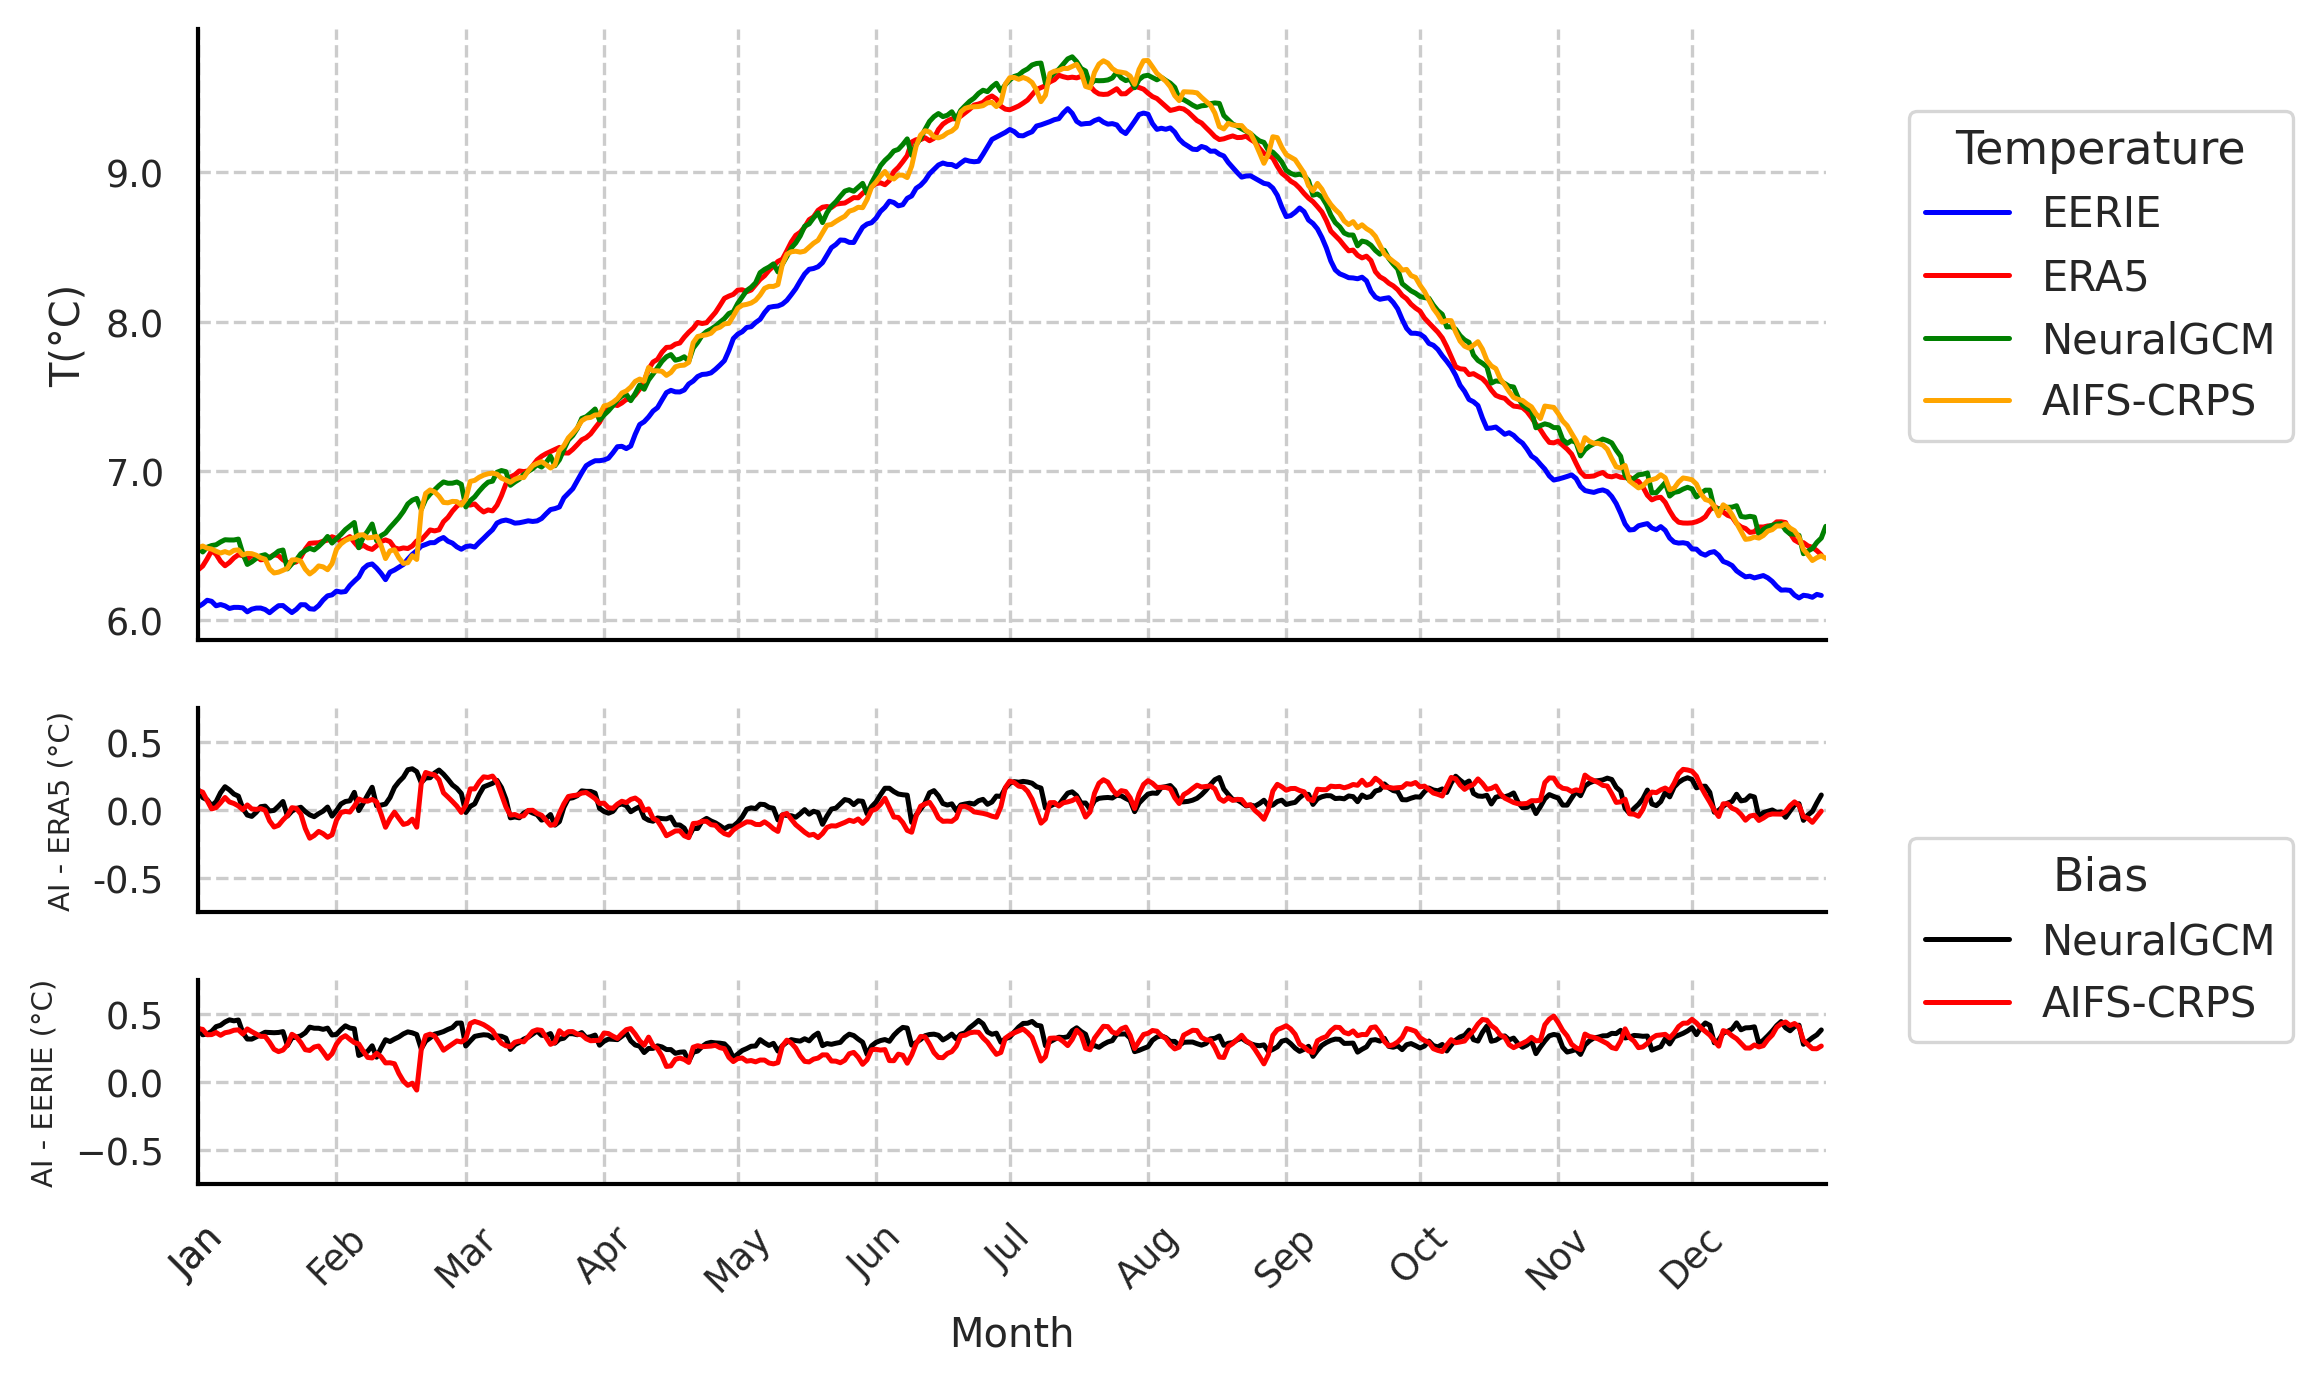
\includegraphics[width=0.8\linewidth]{Chapter2//Figs/climatologie_lines.png}
    \caption{Climatological annual cycle of air temperature at 850~hPa over the period 1981--1990. The upper panel compares the daily climatologies produced by EERIE, ERA5, NeuralGCM, and AIFS-CRPS. For the AI weather models, the climatology is computed using forecast lead times between 10 and 20 days. This interval is selected heuristically to represent the window between the decay of the influence of the initial conditions and the point at which the forecasts begin to lose stability. The middle and lower panels show the temperature differences of the two AI-based models relative to ERA5 and EERIE, respectively.}
    \label{fig:climatology-lines}
\end{figure}

The lead-time-dependent biases in Figure~\ref{fig:climatology-bias} show how this departure develops. NeuralGCM exhibits a predominantly positive bias relative to EERIE-AMIP from the first five-day window onwards. The annual mean bias increases during the initial forecast stages and subsequently remains around $+0.3$--$0.4\,^{\circ}\mathrm{C}$. Relative to ERA5, the annual mean bias is substantially smaller and remains slightly positive after the first five days. Monthly differences nevertheless reveal a seasonal structure, with larger warm biases towards the end of the year. NeuralGCM therefore maintains a comparatively stable global mean over the 30-day integration, but this mean differs systematically from that of EERIE-AMIP.

AIFS-CRPS initially follows a similar pattern, with a small annual mean bias relative to ERA5 and a positive bias relative to EERIE-AMIP. After approximately 20 days, however, its behaviour changes. A cold bias develops, particularly between May and September, and intensifies in the final forecast window. By days 25--30, the annual mean bias is approximately $-0.5\,^{\circ}\mathrm{C}$ relative to ERA5 and $-0.3\,^{\circ}\mathrm{C}$ relative to EERIE-AMIP, while several monthly biases extend beyond the lower limit of the colour scale. This confirms that the cooling identified in the individual forecasts is a recurring, seasonally dependent feature of the evaluated configuration.

\begin{figure}[H]
    \centering
    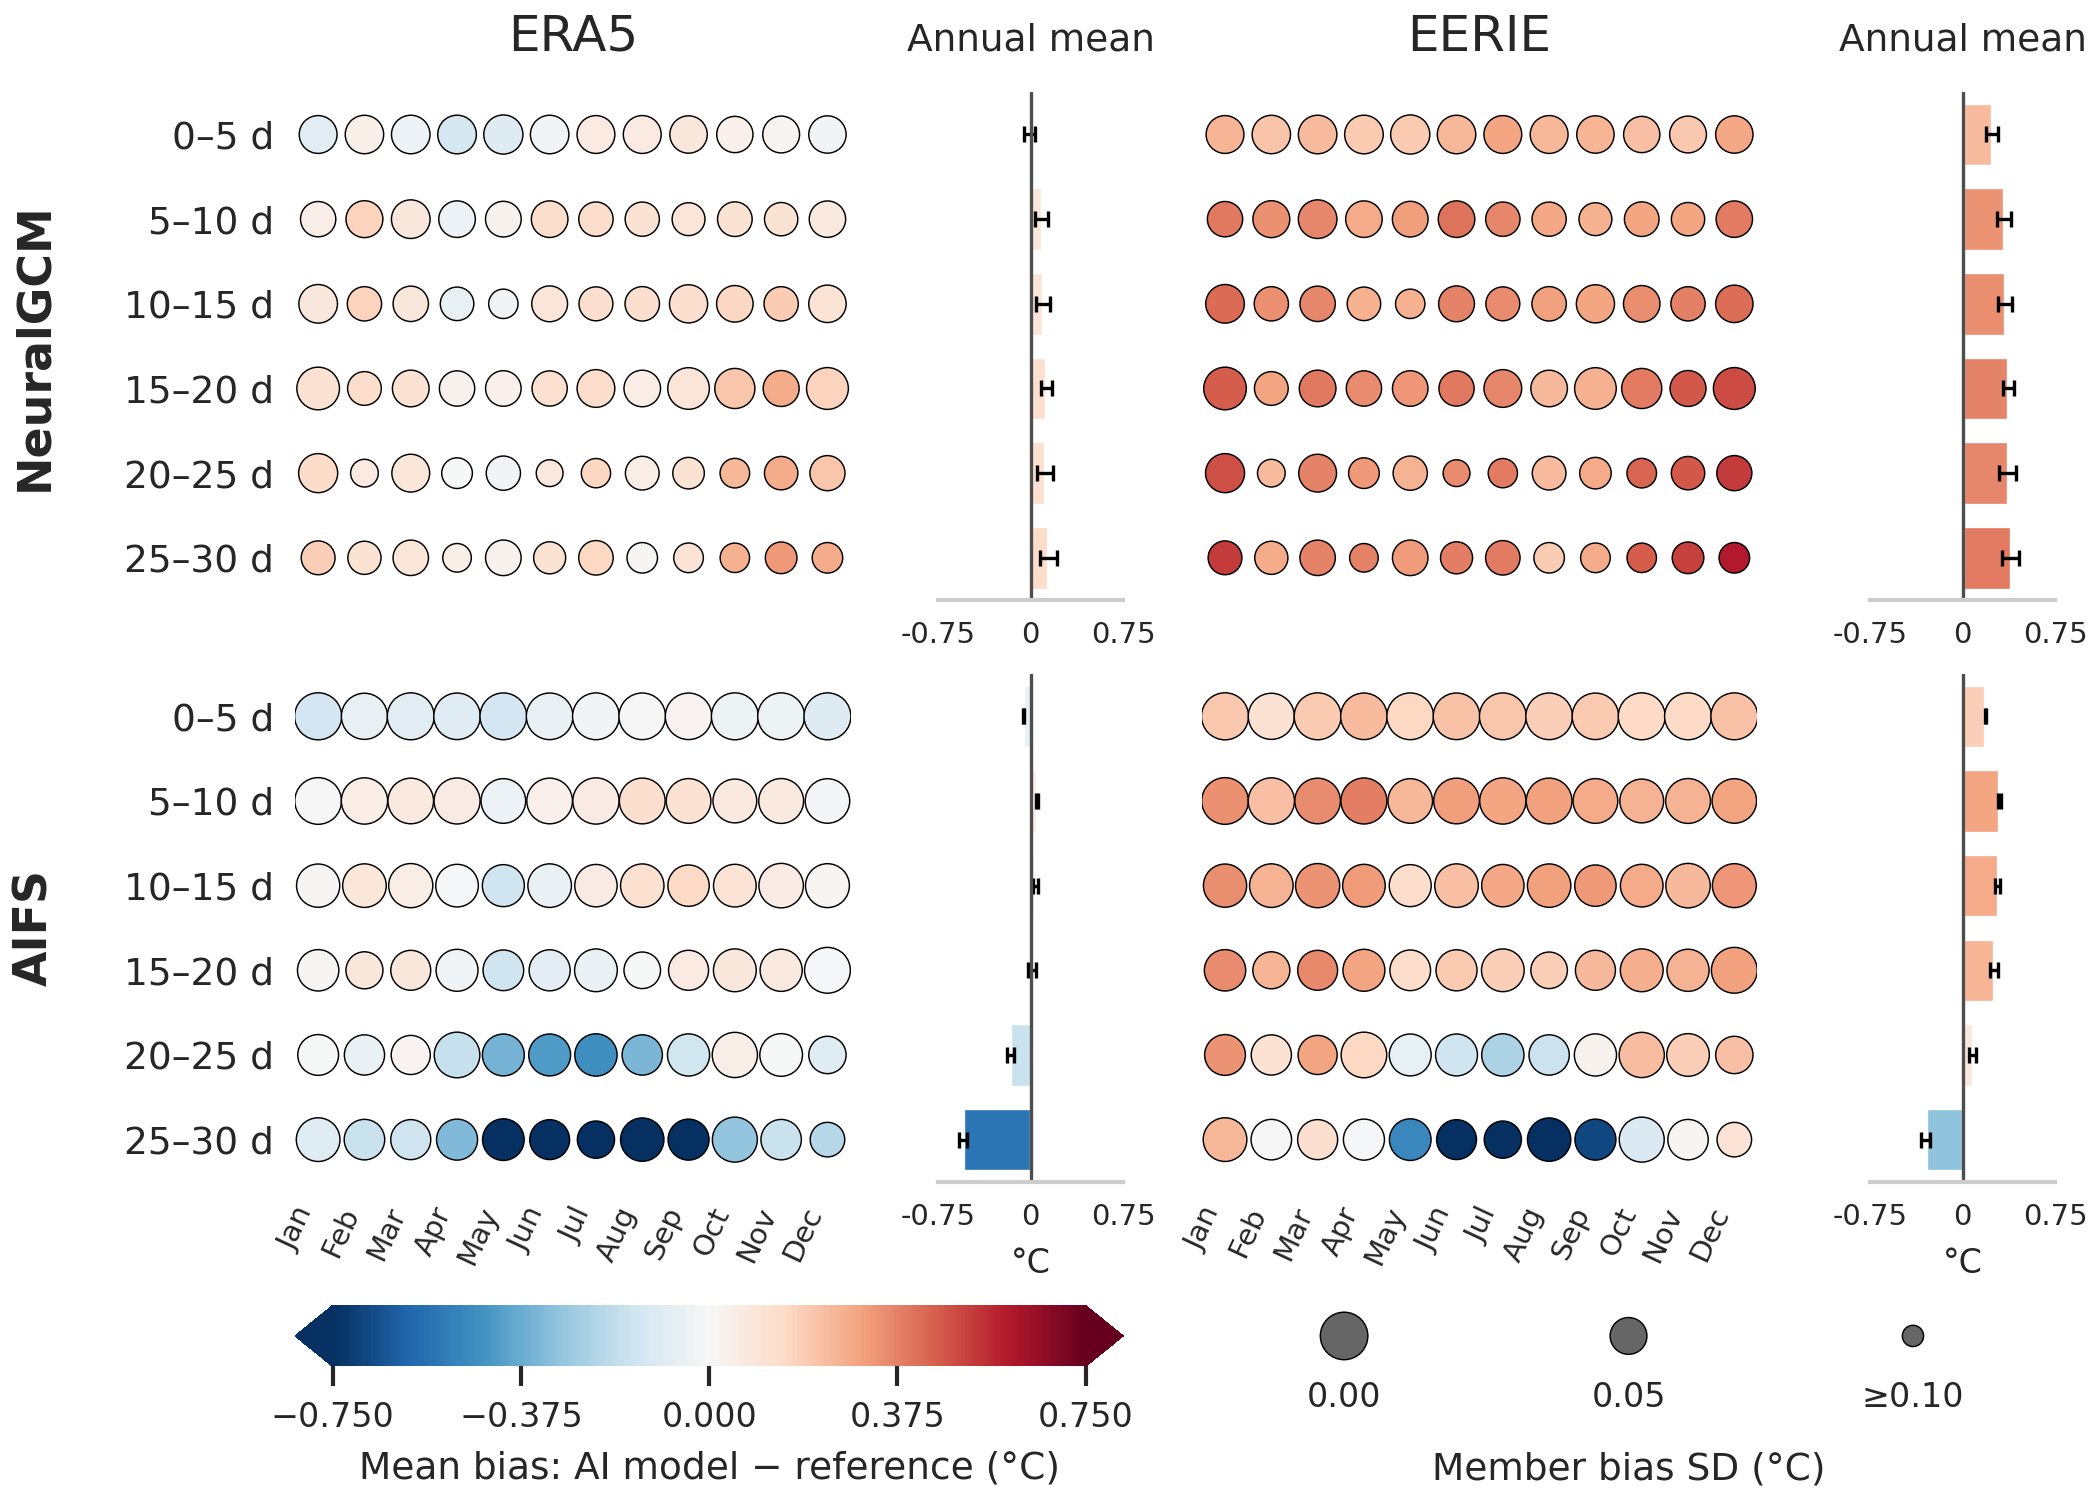
\includegraphics[width=1\linewidth]{Chapter2//Figs/climatologie_bias_vars.png}
    \caption{Climatological bias in global mean temperature at 850~hPa during 1985--1990. NeuralGCM (top) and AIFS-CRPS (bottom) each use ten-member ensembles initialized from EERIE-AMIP member~1. Columns show comparisons with ERA5 (left) and EERIE-AMIP member~1 (right). Circle colours represent the ensemble mean of the area-weighted global biases (AI model minus reference) for each month and five day lead-time window. Larger circles indicate a smaller inter-member standard deviation of the global bias. Horizontal bars show the equally weighted mean of the twelve monthly biases; error bars indicate $\pm$ the mean of the twelve monthly inter-member standard deviations.}
    \label{fig:climatology-bias}
\end{figure}

The initial movement towards an ERA5-like global mean is consistent with an adjustment towards conditions represented in the training data, although the present diagnostics do not establish its mechanism. Related behaviour was reported by \citet{rackow_robustness_2024}, who found that AI weather models could retain useful forecast skill when initialized in different climate states while developing systematic temperature drift towards their training climate. Their experiments concerned colder and warmer climate regimes, whereas the present comparison concerns two representations of the same historical period. Nevertheless, both illustrate why forecast skill and preservation of the source climate must be evaluated separately.

The spatial RMSE provides a further distinction between agreement in the global mean and agreement in the geographical temperature distribution (Figure~\ref{fig:climatology-rmse}). Relative to ERA5, NeuralGCM maintains an annual mean spatial RMSE of approximately $1.1$--$1.3\,^{\circ}\mathrm{C}$ across the forecast windows, despite its much smaller global mean bias. Relative to EERIE-AMIP, RMSE increases from approximately $0.7\,^{\circ}\mathrm{C}$ during days 0--5 to around $1.4\,^{\circ}\mathrm{C}$ during days 25--30. Thus, the relatively stable global mean does not imply preservation of the reference spatial climatology: regional differences remain substantial and can compensate when averaged globally.

AIFS-CRPS shows a broadly comparable spatial RMSE during the first 20 days, followed by a marked deterioration. During days 25--30, the annual mean RMSE reaches approximately $2.5\,^{\circ}\mathrm{C}$ relative to ERA5 and $2.7\,^{\circ}\mathrm{C}$ relative to EERIE-AMIP. The largest monthly errors occur during boreal summer and early autumn, matching the seasonal structure of the cold bias. These changes are much larger than the inter-member variation of the aggregated diagnostics, indicating that the deterioration is shared across the ensemble. 

The results therefore support the use of the 10--20-day interval as a pragmatic window for comparing the generated mean states, after the initial adjustment and before the strongest AIFS-CRPS deterioration. They do not demonstrate complete loss of initialization influence or convergence to an equilibrium climate. Published experiments have shown that selected NeuralGCM configurations can reproduce climate statistics in multi-decadal integrations \citep{kochkov_neural_2024}, while AIFS-CRPS has demonstrated skill in 46-day forecasts initialized from ERA5 \citep{lang_aifs-crps_2026}. These capabilities cannot be transferred automatically to a different initialization source. 

\begin{figure}[H]
    \centering
    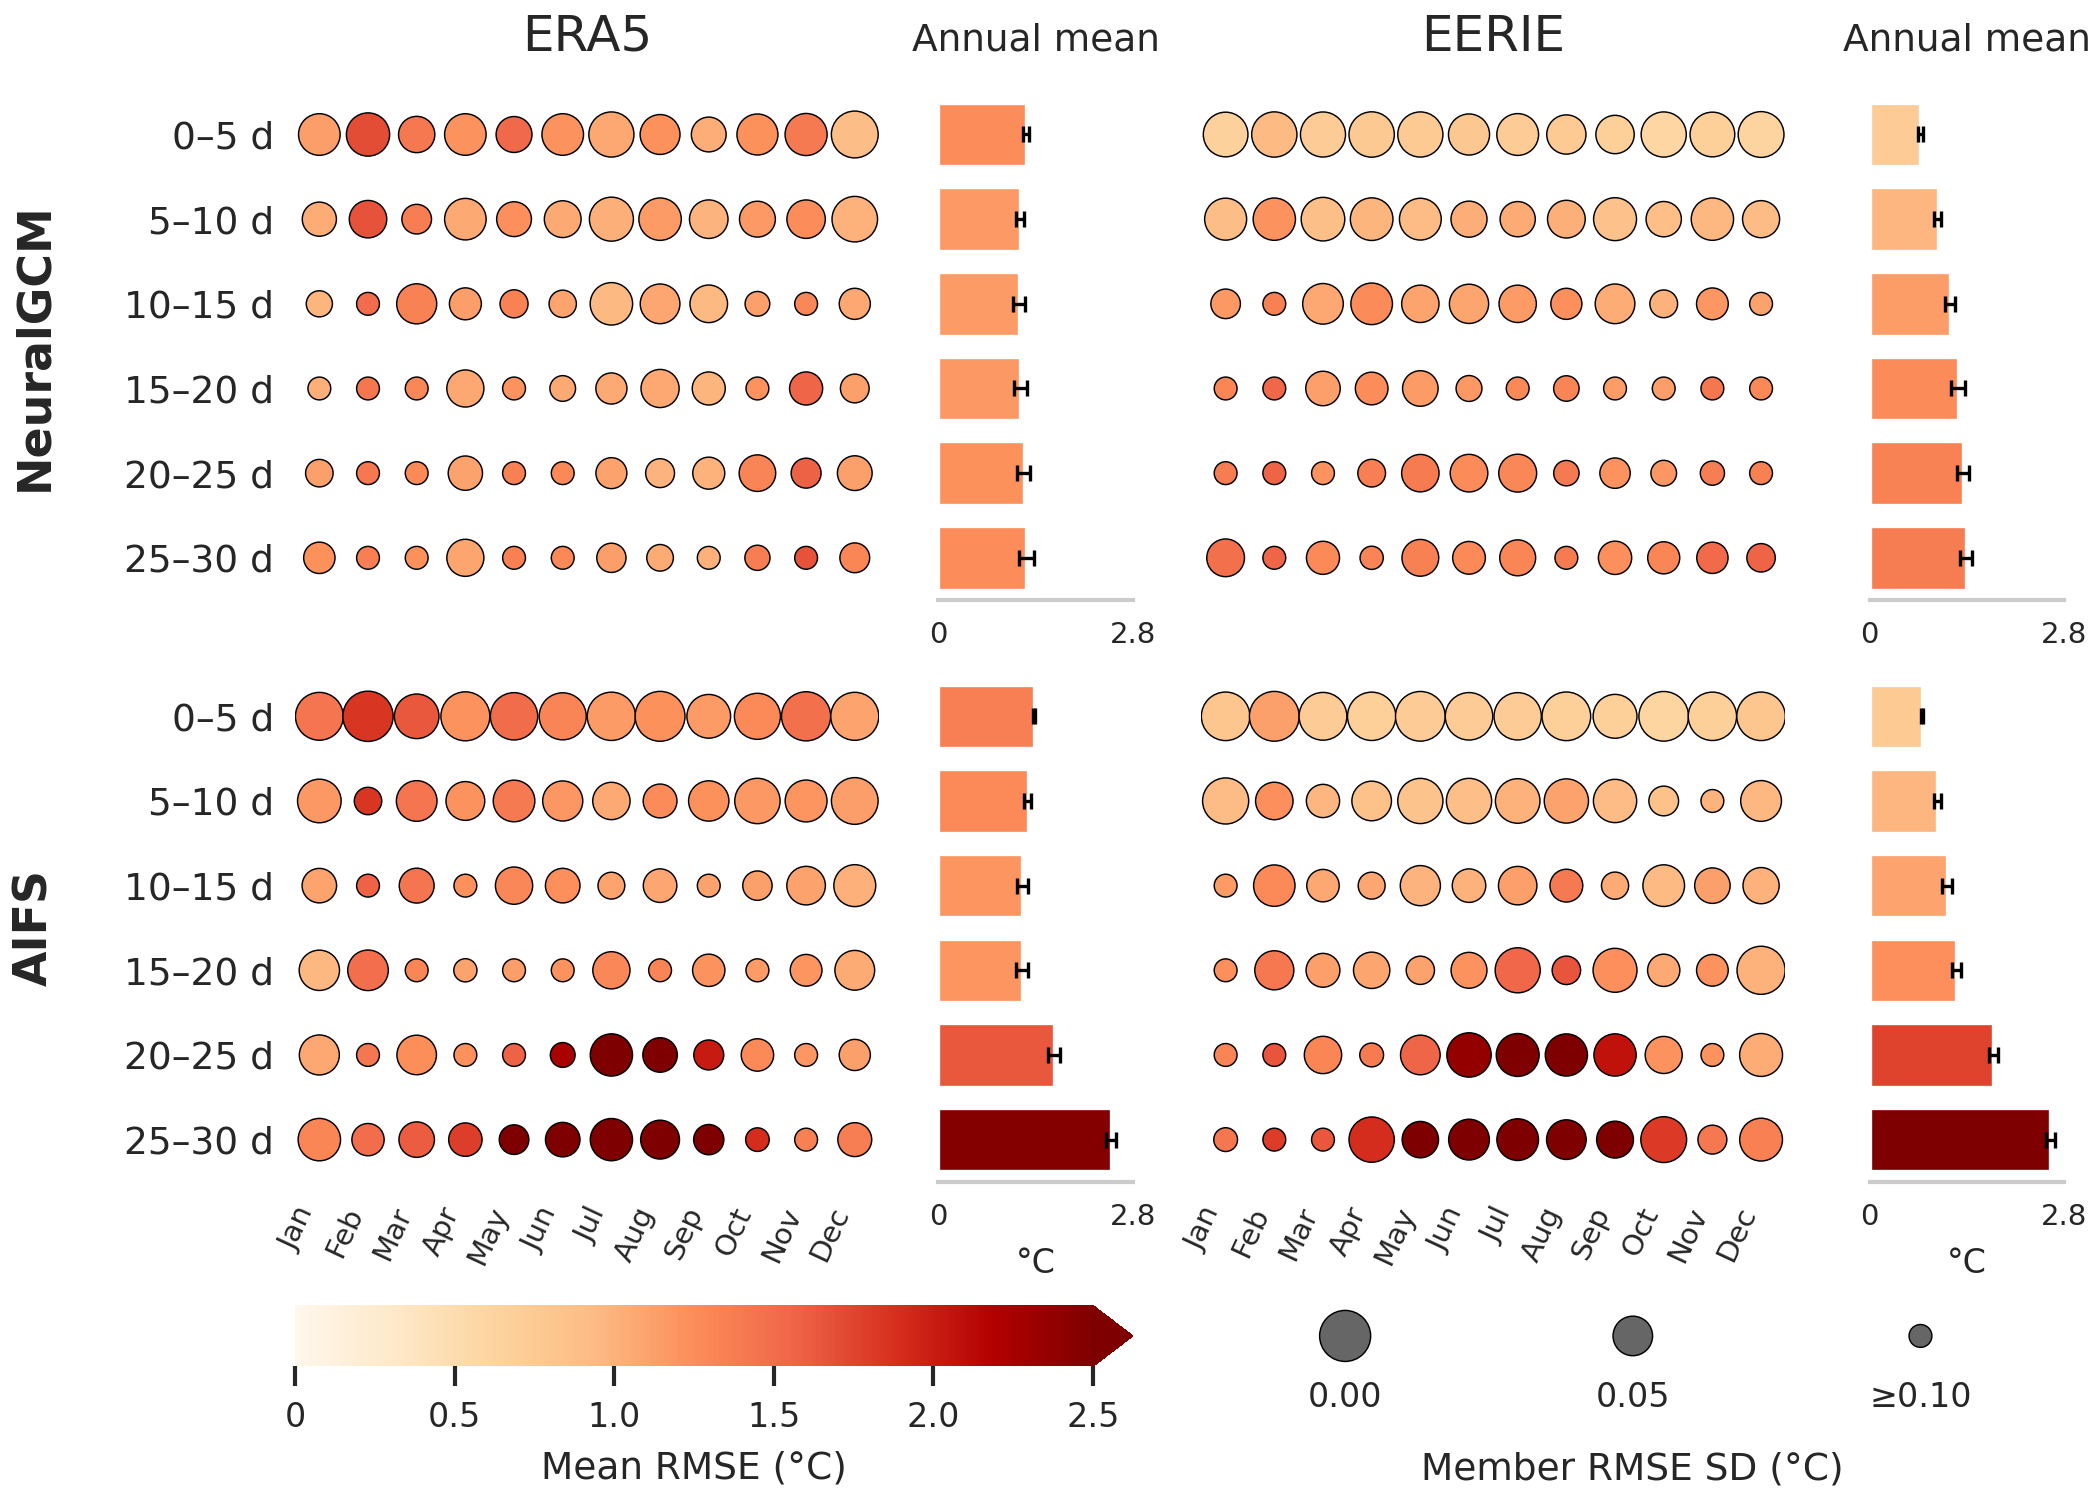
\includegraphics[width=1\linewidth]{Chapter2//Figs/climatologie_rmse_vars.png}
    \caption{Spatial RMSE of monthly climatological temperature fields at 850~hPa during 1985--1990. NeuralGCM (top) and AIFS-CRPS (bottom) each use ten-member ensembles initialized from EERIE-AMIP member~1. Columns show comparisons with ERA5 (left) and EERIE-AMIP member~1 (right). Circle colours represent the mean RMSE across ensemble members for each month and five-day lead-time window, with the spatial RMSE calculated separately for each member before averaging. Larger circles indicate a smaller inter-member standard deviation of the RMSE. Horizontal bars show the equally weighted mean of the twelve monthly RMSE values; error bars indicate $\pm$ the mean of the twelve monthly inter-member standard deviations.}
    \label{fig:climatology-rmse}
\end{figure}

\subsection{Anomalies and Variability}

\section{Discussion}